% !TeX program = xelatex
% Document de passation : données, prétraitement et construction des variables.
% Avant compilation, générer les données du graphique (depuis la racine du projet) :
%   .venv\Scripts\python.exe docs/latex/generer_figures.py
% Compilation depuis docs/latex/ (deux passes, pour les renvois et le bandeau) :
%   xelatex -interaction=nonstopmode -halt-on-error -output-directory=build Passation_donnees_et_variables.tex
\documentclass[10pt,a4paper]{article}
\usepackage[left=15mm,right=15mm,top=14mm,bottom=17mm,footskip=8mm]{geometry}
\usepackage{amsmath}
\usepackage{unicode-math}
\setmainfont{Calibri}
\setmathfont{Cambria Math}
\usepackage[table]{xcolor}
\usepackage{array,tabularx,booktabs,longtable}
\setlength{\LTleft}{0pt}\setlength{\LTright}{0pt}
\setlength{\LTpre}{3pt}\setlength{\LTpost}{2pt}
\usepackage{enumitem}
\usepackage{titlesec}
\usepackage{fancyhdr}
\usepackage{tikz}
\usetikzlibrary{arrows.meta,positioning,calc}
\usepackage[skins,breakable,raster]{tcolorbox}
\usepackage{fontawesome5}
\usepackage{hyperref}

% ---------------------------------------------------------------- Couleurs
\definecolor{marine}{HTML}{16324A}
\definecolor{sarcelle}{HTML}{087F83}
\definecolor{orange}{HTML}{C9731C}
\definecolor{rouge}{HTML}{B23A48}
\definecolor{vert}{HTML}{2E7D4F}
\definecolor{gris}{HTML}{F2F5F7}
\definecolor{texte}{HTML}{22313F}
\definecolor{discret}{HTML}{5F7381}
\color{texte}
\hypersetup{colorlinks=true,urlcolor=sarcelle,linkcolor=sarcelle,citecolor=sarcelle,
  pdftitle={Passation n°1 : données, prétraitement et construction des variables},
  pdfauthor={Mamadou Cherif DIALLO}, pdfsubject={Projet de machine learning, M2 Finance de marché et gestion des risques, Paris 1}}

% ---------------------------------------------------------------- Mise en page
\setlength{\parindent}{0pt}
\setlength{\parskip}{4.5pt}
\linespread{1.04}
\setlength{\emergencystretch}{2em}
\setlist{nosep,leftmargin=1.4em,topsep=2pt,itemsep=1.5pt}
\setlist[itemize]{label={\color{sarcelle}\small\faIcon{caret-right}}}
\renewcommand{\arraystretch}{1.22}
\newcolumntype{Y}{>{\raggedright\arraybackslash}X}
\newcolumntype{L}[1]{>{\raggedright\arraybackslash}p{#1}}
\newcommand{\entete}[1]{\textcolor{white}{\bfseries #1}}

\titleformat{\section}{\Large\bfseries\color{marine}}
  {\tikz[baseline=(n.base)]\node[fill=sarcelle,text=white,rounded corners=2pt,inner sep=3pt,font=\large\bfseries](n){\thesection};}
  {0.55em}{}[\vspace{-3pt}{\color{sarcelle!35}\titlerule[0.7pt]}]
\titleformat{\subsection}{\large\bfseries\color{sarcelle}}{\thesubsection}{0.5em}{}
\titlespacing*{\section}{0pt}{9pt}{4pt}
\titlespacing*{\subsection}{0pt}{5pt}{1pt}

% Garde un titre avec la suite de son contenu (équivalent de needspace).
\makeatletter
\newcommand{\besoin}[1]{\par\penalty-100\begingroup\setlength{\dimen@}{#1}%
  \dimen@ii\pagegoal\advance\dimen@ii-\pagetotal
  \ifdim\dimen@>\dimen@ii\ifdim\dimen@ii>\z@\vfil\fi\break\fi\endgroup}
\makeatother
\let\sectionorigine\section
\renewcommand{\section}{\besoin{6\baselineskip}\sectionorigine}
\let\soussectionorigine\subsection
\renewcommand{\subsection}{\besoin{5\baselineskip}\soussectionorigine}
\renewcommand{\refname}{Références}

\pagestyle{fancy}\fancyhf{}
\renewcommand{\headrulewidth}{0pt}
\renewcommand{\footrulewidth}{0pt}
\fancyfoot[L]{\footnotesize\color{discret}\textcolor{sarcelle}{\faIcon{folder-open}}\enspace Passation n\textsuperscript{o}\,1 — Données, prétraitement et variables\enspace·\enspace Master 2, Paris 1}
\fancyfoot[R]{\footnotesize\color{discret}\thepage\,/\,\pageref{derniere}}

% ---------------------------------------------------------------- Encadrés
\tcbset{
  base/.style={enhanced,breakable,colback=#1!5,colframe=#1,boxrule=0pt,leftrule=3pt,
    arc=1.5pt,outer arc=1.5pt,left=7pt,right=7pt,top=3pt,bottom=3pt,before skip=5pt,after skip=5pt,
    fonttitle=\bfseries,coltitle=#1,colbacktitle=#1!5,titlerule=0pt,toptitle=3pt,bottomtitle=-1pt},
  tuile/.style={enhanced,colback=white,colframe=sarcelle!40,boxrule=0.6pt,arc=3pt,
    halign=center,valign=center,top=3pt,bottom=3pt,left=2pt,right=2pt}}
\newtcolorbox{formule}[1]{base=sarcelle,title={\faIcon{square-root-alt}\enspace #1}}
\newtcolorbox{fournisseur}[1]{base=discret,title={\faIcon{building}\enspace #1}}
\newtcolorbox{retenir}[1]{base=marine,title={\faIcon{lightbulb}\enspace #1}}
\newtcolorbox{attention}[1]{base=orange,title={\faIcon{exclamation-triangle}\enspace #1}}
\newtcolorbox{correction}[1]{base=rouge,title={\faIcon{tools}\enspace #1}}
\newtcolorbox{valide}[1]{base=vert,title={\faIcon{check-circle}\enspace #1}}

% Nom de fichier ou de colonne : police à chasse fixe, coupure de ligne permise après chaque « _ ».
\newcommand{\coupure}{\textunderscore\allowbreak}
\newcommand{\fic}[1]{{\small\ttfamily\let\_\coupure #1}}
\newcommand{\fait}{\textcolor{vert}{\faIcon{check-circle}\ fait}}
\newcommand{\afaire}{\textcolor{orange}{\faIcon{hourglass-half}\ à faire}}
\newcommand{\enpartie}{\textcolor{sarcelle}{\faIcon{adjust}\ en partie}}
\newcommand{\SPY}{\mathrm{SPY}}
\newcommand{\IEF}{\mathrm{IEF}}
% Légende d'un symbole : \notation{symbole}{nom et signification}
\newcommand{\notation}[2]{\makebox[2.3cm][l]{#1}\parbox[t]{\dimexpr\linewidth-2.3cm\relax}{#2}\par}

% Fichier généré par generer_figures.py : ne pas modifier à la main.
\newcommand{\tracecible}[1]{\draw[#1] plot coordinates {(0.0000,4.34) (0.0833,5.45) (0.1667,6.74) (0.2500,6.66) (0.3333,8.75) (0.4167,8.62) (0.5000,6.44) (0.5833,5.59) (0.6667,5.31) (0.7500,7.20) (0.8333,6.18) (0.9167,6.74) (1.0000,4.81) (1.0833,5.58) (1.1667,6.30) (1.2500,6.25) (1.3333,8.90) (1.4167,9.19) (1.5000,5.80) (1.5833,6.69) (1.6667,7.51) (1.7500,6.47) (1.8333,5.83) (1.9167,5.83) (2.0000,7.70) (2.0833,4.94) (2.1667,6.41) (2.2500,4.98) (2.3333,3.95) (2.4167,3.71) (2.5000,6.10) (2.5833,4.35) (2.6667,8.37) (2.7500,6.45) (2.8333,5.89) (2.9167,7.78) (3.0000,6.64) (3.0833,8.12) (3.1667,7.22) (3.2500,6.81) (3.3333,5.76) (3.4167,6.03) (3.5000,8.01) (3.5833,14.95) (3.6667,9.10) (3.7500,6.98) (3.8333,9.83) (3.9167,10.64) (4.0000,11.58) (4.0833,8.09) (4.1667,5.64) (4.2500,5.35) (4.3333,5.72) (4.4167,8.45) (4.5000,3.42) (4.5833,7.10) (4.6667,6.19) (4.7500,5.26) (4.8333,5.51) (4.9167,3.91) (5.0000,3.41) (5.0833,4.64) (5.1667,3.80) (5.2500,3.74) (5.3333,3.97) (5.4167,4.91) (5.5000,3.97) (5.5833,3.77) (5.6667,2.40) (5.7500,3.34) (5.8333,3.88) (5.9167,4.47) (6.0000,13.57) (6.0833,10.32) (6.1667,11.43) (6.2500,6.88) (6.3333,4.70) (6.4167,4.88) (6.5000,4.48) (6.5833,3.56) (6.6667,8.94) (6.7500,11.71) (6.8333,13.72) (6.9167,13.63) (7.0000,6.82) (7.0833,5.40) (7.1667,4.95) (7.2500,6.63) (7.3333,7.56) (7.4167,5.53) (7.5000,9.40) (7.5833,7.74) (7.6667,6.88) (7.7500,3.89) (7.8333,4.19) (7.9167,4.76) (8.0000,8.83) (8.0833,35.83) (8.1667,35.32) (8.2500,15.39) (8.3333,14.63) (8.4167,11.67) (8.5000,6.64) (8.5833,12.41) (8.6667,11.16) (8.7500,12.49) (8.8333,6.35) (8.9167,6.96) (9.0000,9.85) (9.0833,11.79) (9.1667,7.67) (9.2500,8.25) (9.3333,6.72) (9.4167,5.74) (9.5000,5.12) (9.5833,6.04) (9.6667,8.57) (9.7500,5.71) (9.8333,8.88) (9.9167,9.50) (10.0000,13.14) (10.0833,13.98) (10.1667,12.75) (10.2500,19.18) (10.3333,18.64) (10.4167,14.54) (10.5000,13.28) (10.5833,15.70) (10.6667,19.63) (10.7500,18.66) (10.8333,14.99) (10.9167,12.13) (11.0000,11.21) (11.0833,9.90) (11.1667,7.19) (11.2500,7.27) (11.3333,7.29) (11.4167,7.47) (11.5000,7.88) (11.5833,8.40) (11.6667,9.38) (11.7500,11.18) (11.8333,7.88) (11.9167,7.19) (12.0000,8.44) (12.0833,7.37) (12.1667,7.52) (12.2500,8.85) (12.3333,6.76) (12.4167,6.98) (12.5000,11.54) (12.5833,8.39) (12.6667,5.87) (12.7500,7.76) (12.8333,7.71) (12.9167,10.30) (13.0000,8.06) (13.0833,10.87) (13.1667,25.59) (13.2500,15.73) (13.3333,8.38) (13.4167,6.08) (13.5000,6.08) (13.5833,6.22) (13.6667,6.32) (13.7500,8.07) (13.8333,7.32)};}
\newcommand{\tracevix}[1]{\draw[#1] plot coordinates {(0.0000,20.23) (0.0833,18.42) (0.1667,16.17) (0.2500,17.82) (0.3333,21.00) (0.4167,21.13) (0.5000,17.57) (0.5833,15.69) (0.6667,15.28) (0.7500,16.28) (0.8333,16.70) (0.9167,17.31) (1.0000,13.51) (1.0833,14.07) (1.1667,13.03) (1.2500,13.97) (1.3333,13.49) (1.4167,17.27) (1.5000,13.97) (1.5833,14.21) (1.6667,14.69) (1.7500,15.41) (1.8333,12.92) (1.9167,14.19) (2.0000,14.24) (2.0833,15.47) (2.1667,14.84) (2.2500,14.20) (2.3333,12.48) (2.4167,11.54) (2.5000,12.30) (2.5833,13.49) (2.6667,13.47) (2.7500,18.06) (2.8333,13.41) (2.9167,16.29) (3.0000,19.12) (3.0833,15.90) (3.1667,14.81) (3.2500,13.49) (3.3333,13.34) (3.4167,14.34) (3.5000,14.35) (3.5833,19.43) (3.6667,24.38) (3.7500,16.79) (3.8333,16.21) (3.9167,18.03) (4.0000,23.72) (4.0833,22.52) (4.1667,15.85) (4.2500,14.30) (4.3333,14.85) (4.4167,17.77) (4.5000,13.16) (4.5833,12.40) (4.6667,14.22) (4.7500,14.59) (4.8333,15.24) (4.9167,12.47) (5.0000,11.61) (5.0833,11.53) (5.1667,11.90) (5.2500,13.14) (5.3333,10.86) (5.4167,10.51) (5.5000,10.26) (5.5833,11.98) (5.6667,10.44) (5.7500,10.13) (5.8333,10.54) (5.9167,10.26) (6.0000,11.06) (6.0833,22.46) (6.1667,19.02) (6.2500,18.27) (6.3333,14.12) (6.4167,13.68) (6.5000,13.15) (6.5833,12.55) (6.6667,12.91) (6.7500,19.35) (6.8333,19.39) (6.9167,24.95) (7.0000,19.57) (7.0833,15.23) (7.1667,14.49) (7.2500,12.95) (7.3333,16.72) (7.4167,15.84) (7.5000,13.31) (7.5833,18.98) (7.6667,15.56) (7.7500,15.47) (7.8333,12.52) (7.9167,13.76) (8.0000,13.94) (8.0833,19.63) (8.1667,57.74) (8.2500,41.45) (8.3333,30.90) (8.4167,31.12) (8.5000,26.84) (8.5833,22.89) (8.6667,27.65) (8.7500,29.44) (8.8333,25.00) (8.9167,22.37) (9.0000,24.91) (9.0833,23.14) (9.1667,21.84) (9.2500,17.42) (9.3333,19.76) (9.4167,16.96) (9.5000,17.60) (9.5833,17.47) (9.6667,19.82) (9.7500,17.87) (9.8333,18.50) (9.9167,21.35) (10.0000,23.18) (10.0833,25.75) (10.1667,26.97) (10.2500,24.37) (10.3333,29.45) (10.4167,28.10) (10.5000,24.87) (10.5833,22.17) (10.6667,27.41) (10.7500,30.01) (10.8333,23.44) (10.9167,21.78) (11.0000,20.20) (11.0833,20.06) (11.1667,21.64) (11.2500,17.82) (11.3333,17.64) (11.4167,13.99) (11.5000,13.94) (11.5833,15.85) (11.6667,15.24) (11.7500,18.89) (11.8333,14.08) (11.9167,12.72) (12.0000,13.40) (12.0833,13.94) (12.1667,13.79) (12.2500,16.14) (12.3333,13.09) (12.4167,12.68) (12.5000,14.47) (12.5833,19.31) (12.6667,17.77) (12.7500,19.96) (12.8333,16.12) (12.9167,15.87) (13.0000,16.75) (13.0833,17.05) (13.1667,21.84) (13.2500,31.97) (13.3333,20.46) (13.4167,18.21) (13.5000,16.33) (13.5833,15.75) (13.6667,15.77) (13.7500,18.09) (13.8333,19.90) (13.9167,15.55)};}


\begin{document}

% ================================================================ Bandeau de titre
\thispagestyle{fancy}
\begin{tikzpicture}[remember picture,overlay]
  \fill[marine] (current page.north west) rectangle ([yshift=-4.6cm]current page.north east);
  \fill[sarcelle] ([yshift=-4.6cm]current page.north west) rectangle ([yshift=-4.85cm]current page.north east);
  \node[anchor=north west,text=white,align=left,text width=17.5cm] at ([xshift=15mm,yshift=-11mm]current page.north west)
    {{\small\bfseries\color{sarcelle!40!white}PROJET DE MACHINE LEARNING\enspace·\enspace M2 FINANCE DE MARCHÉ ET GESTION DES RISQUES\enspace·\enspace PARIS 1}\\[7pt]
     {\fontsize{22}{26}\selectfont\bfseries Passation n\textsuperscript{o}\,1 : données, prétraitement\\[3pt] et construction des variables}\\[7pt]
     {\normalsize Prévision du risque d'un portefeuille actions–obligations et apport de l'information des options}};
  \node[anchor=south east,text=white!85!marine,align=right,font=\small] at ([xshift=-15mm,yshift=-4.35cm]current page.north east)
    {Mamadou Cherif DIALLO\enspace·\enspace 21 novembre 2026\\ Cours \emph{Introduction to Machine Learning} — M.~El Fakir, N.~de Roux};
\end{tikzpicture}
\vspace*{4.05cm}

\begin{retenir}{En une minute}
J'ai collecté 29 sources de marché et je les ai alignées sur le calendrier de la Bourse de New York. J'ai ensuite construit la \textbf{cible} à prévoir : la volatilité du panier composé à 60\,\% de l'ETF actions SPY et à 40\,\% de l'ETF obligataire IEF, mesurée sur les 21 séances suivantes. J'ai aussi construit deux familles de variables explicatives : les \textbf{13 variables historiques (A)} et les \textbf{8 indicateurs tirés des options (B)}. Chaque chiffre se recalcule avec trois scripts et est contrôlé par 7 tests et un audit indépendant de 48 contrôles. Aucun modèle n'est encore entraîné. Ce document explique, pour chaque donnée, \emph{ce qu'elle est}, \emph{comment elle est calculée} et \emph{sous quelles hypothèses}, pour que vous repreniez à l'étape d'exploration (section~\ref{sec:suite}).
\end{retenir}

\begin{tcbraster}[raster columns=4,raster equal height,raster column skip=6pt,raster before skip=2pt,raster after skip=4pt]
\begin{tcolorbox}[tuile]{\color{sarcelle}\Large\faIcon{calendar-alt}}\\[2pt]{\Large\bfseries\color{marine}3\,520}\\{\small séances, 2012–2025}\end{tcolorbox}
\begin{tcolorbox}[tuile]{\color{sarcelle}\Large\faIcon{database}}\\[2pt]{\Large\bfseries\color{marine}29}\\{\small fichiers de données, 8 fournisseurs}\end{tcolorbox}
\begin{tcolorbox}[tuile]{\color{sarcelle}\Large\faIcon{layer-group}}\\[2pt]{\Large\bfseries\color{marine}13 + 8}\\{\small variables A et B}\end{tcolorbox}
\begin{tcolorbox}[tuile]{\color{sarcelle}\Large\faIcon{clipboard-check}}\\[2pt]{\Large\bfseries\color{marine}7 + 48}\\{\small tests et contrôles d'audit}\end{tcolorbox}
\end{tcbraster}

\textbf{Comment lire ce document.} Les nombres entre crochets, comme [23], renvoient à la liste des \textbf{références} à la fin du document : la source ou l'article d'où vient l'information (ils sont cliquables). Les formules sont numérotées (1), (2)… et portent un nom ; leur liste complète est en annexe~\ref{sec:equations}. Sous chaque formule, une légende définit \emph{chaque} symbole. Les abréviations sont définies à la section~\ref{sec:abreviations}, les colonnes des fichiers dans les fiches de l'annexe~\ref{sec:fiches} et les symboles dans l'index de l'annexe~\ref{sec:symboles}. Code couleur des encadrés : \textcolor{sarcelle}{\textbf{vert d'eau}}, nos formules ; \textcolor{discret}{\textbf{gris}}, les calculs d'un fournisseur ; \textcolor{marine}{\textbf{bleu}}, à retenir ; \textcolor{orange}{\textbf{orange}}, points d'attention ; \textcolor{rouge}{\textbf{rouge}}, corrections ; \textcolor{vert}{\textbf{vert}}, contrôles validés.

% ================================================================
\section{Abréviations et vocabulaire}\label{sec:abreviations}
{\small
\begin{longtable}{@{}>{\leavevmode\bfseries\color{marine}}L{1.75cm} L{6.6cm} >{\leavevmode\bfseries\color{marine}}L{1.75cm} L{6.6cm}@{}}
\rowcolor{marine}\entete{Sigle} & \entete{Signification} & \entete{Sigle} & \entete{Signification} \\
\endhead
AM & \emph{Ante Meridiem}, « le matin » : option réglée sur un cours de l'indice calculé à l'\textbf{ouverture} du jour d'échéance ; elle ne se négocie plus dès la veille au soir. Cas des options SPX mensuelles. Voir PM. & NAV & \emph{Net Asset Value}, en français \textbf{valeur liquidative} : ce que vaut réellement une part du fonds, calculée chaque soir par le gestionnaire, soit (valeur des titres détenus − dettes) / nombre de parts. Elle reste très proche du cours en Bourse ; je m'en sers pour contrôler les prix de Yahoo. \\
\rowcolor{gris}ATM & \emph{At The Money}, « à la monnaie » : prix d'exercice égal au cours du sous-jacent & NYSE & \emph{New York Stock Exchange} ; son code de marché est XNYS \\
bid / ask & meilleur prix d'achat / de vente proposé sur le marché ; leur écart est la fourchette & OTM & \emph{Out of The Money}, « hors de la monnaie » : put sous le cours, call au-dessus \\
\rowcolor{gris}Cboe & \emph{Chicago Board Options Exchange}, Bourse d'options qui calcule le VIX & pb (bp) & point de base : 0,01\,\% = 0,0001 \\
CRSP & \emph{Center for Research in Security Prices}, base de prix de référence (Chicago) & PM & \emph{Post Meridiem}, « l'après-midi » : option réglée sur le cours de \textbf{clôture} de l'indice le jour d'échéance ; elle se négocie jusqu'à cette clôture. Cas des SPXW. Je n'utilise que des options PM, pour ne pas mélanger les deux règles. \\
\rowcolor{gris}DTE & \emph{Days To Expiration}, jours calendaires restant jusqu'à l'échéance & QLIKE & perte « quasi-vraisemblance » pour juger une prévision de variance (équation~\ref{eq:metriques}) \\
EOD & \emph{End Of Day}, données de fin de journée & RF & \emph{Risk-Free}, rendement des liquidités sans risque \\
\rowcolor{gris}ET & \emph{Eastern Time}, heure de New York & RMSE & \emph{Root Mean Squared Error}, racine de l'erreur quadratique moyenne \\
ETF & \emph{Exchange-Traded Fund}, fonds indiciel coté, négocié comme une action & S\&P~500 & indice des 500 grandes capitalisations américaines (Standard \& Poor's) \\
\rowcolor{gris}EWMA & \emph{Exponentially Weighted Moving Average}, moyenne à pondération exponentielle & SKEW & indice d'asymétrie de Cboe (équation~\ref{eq:skewcboe}) \\
GARCH & \emph{Generalized AutoRegressive Conditional Heteroskedasticity}, modèle de variance \cite{bollerslev} & SPX & code de l'indice S\&P~500 et de ses options européennes (Yahoo : \texttt{\textasciicircum GSPC}) \\
\rowcolor{gris}ICE BofA & indice de T-bills d'\emph{Intercontinental Exchange} et \emph{Bank of America} & SPXW & \emph{SPX Weeklys}, « SPX hebdomadaires » : options sur le S\&P~500 qui arrivent à échéance très souvent (chaque semaine, et aujourd'hui chaque jour de Bourse), au lieu d'une fois par mois. Elles sont réglées PM, sur la clôture du jour d'échéance. \\
IEF & \emph{iShares 7–10 Year Treasury Bond ETF} : ETF d'obligations d'État américaines de 7 à 10 ans & SPY & \emph{SPDR S\&P 500 ETF Trust} : ETF qui réplique le S\&P~500 (SPDR = \emph{Standard \& Poor's Depositary Receipts}) \\
\rowcolor{gris}ITM & \emph{In The Money}, « dans la monnaie » : put au-dessus du cours, call en dessous & SVI & \emph{Stochastic Volatility Inspired} : formule à 5 paramètres qui dessine le \textbf{sourire de volatilité}, c'est-à-dire la courbe des volatilités implicites selon le prix d'exercice, souvent en forme de U penché. On choisit ses paramètres pour qu'elle passe au plus près des cotations du jour, ce qui lisse les données \cite{gatheraljacquier}. \\
IV & \emph{Implied Volatility}, volatilité implicite : volatilité qui, dans le modèle de Black-Scholes, redonne le prix observé d'une option & T-bill & \emph{Treasury bill}, bon du Trésor américain à moins d'un an, sans coupon \\
\rowcolor{gris}K/S & \emph{moneyness} : prix d'exercice rapporté au cours du sous-jacent & UTC & temps universel coordonné \\
MAE & \emph{Mean Absolute Error}, erreur absolue moyenne & VIX, VIX9D, VIX3M, VIX6M & indices de volatilité de Cboe à 30 jours, 9 jours, 3 mois, 6 mois (équations~\ref{eq:vix}–\ref{eq:vix30}) \\
\rowcolor{gris}MLP & \emph{Multilayer Perceptron}, réseau de neurones dense & XGBoost & \emph{eXtreme Gradient Boosting}, arbres de décision ajoutés successivement \\
NaN & \emph{Not a Number} : case vide, valeur manquante & & \\
\end{longtable}}

\textbf{Vocabulaire des options.}
\begin{itemize}
\item Un \textbf{call} (\textbf{put}) européen donne le droit d'acheter (de vendre) l'indice au \textbf{prix d'exercice} $K$ (\emph{strike}) à l'\textbf{échéance} $T$, et seulement à cette date.
\item Le \textbf{règlement} (\emph{settlement}) est le dénouement de l'option à l'échéance. Les options SPX sont \textbf{réglées en espèces} : aucune action n'est livrée. Le détenteur reçoit $100\,\$\times\max(S_{\mathrm{règ}}-K,\,0)$ pour un call et $100\,\$\times\max(K-S_{\mathrm{règ}},\,0)$ pour un put, où $S_{\mathrm{règ}}$ est le \textbf{cours de règlement} de l'indice et 100~\$ le multiplicateur du contrat. Ce cours est fixé soit à l'ouverture (règlement \textbf{AM}), soit à la clôture (règlement \textbf{PM}) du jour d'échéance : voir le tableau ci-dessus. Un \textbf{straddle} est l'achat simultané d'un call et d'un put de même prix d'exercice : il gagne si l'indice bouge fortement, dans un sens ou dans l'autre.
\item Le prix d'une option se décompose en deux morceaux. La \textbf{valeur intrinsèque} est ce que l'option rapporterait si on l'exerçait aujourd'hui ; elle se calcule sans rien deviner. La \textbf{valeur temps} est le reste, ce qu'on paie en plus parce que l'indice peut encore bouger d'ici l'échéance. \textbf{Seule la valeur temps contient l'information de volatilité.} Exemple du 1\textsuperscript{er} juillet 2022, avec le S\&P~500 à 3\,825 et un prix d'exercice de 3\,450 : le call vaut 382 = 375 de valeur intrinsèque (acheter à 3\,450 ce qui vaut 3\,825) + 7 de valeur temps ; le put vaut 9 = 0 de valeur intrinsèque + 9 de valeur temps. Une option dont la valeur intrinsèque est nulle est dite \textbf{hors de la monnaie} (OTM) : c'est le put quand le prix d'exercice est sous le cours, le call quand il est au-dessus.
\item Une \textbf{chaîne d'options} est la liste de toutes les options cotées un jour donné sur un même indice : tous les prix d'exercice et toutes les échéances, calls et puts, chacun avec son prix d'achat et son prix de vente. Pour le S\&P~500, une chaîne compte environ 20\,000 contrats par jour. Les options du S\&P~500 portent le code \textbf{SPX} (échéances mensuelles) ou \textbf{SPXW} (échéances hebdomadaires).
\item La \textbf{volatilité} d'un actif (SPY, IEF, le panier ou l'indice S\&P~500) mesure l'ampleur des variations de son \textbf{prix d'une séance à l'autre}, à la hausse comme à la baisse. C'est l'écart-type de ses rendements quotidiens, ramené à l'année. Par exemple, une volatilité de 16\,\% par an signifie que le prix varie typiquement d'environ $16\,\%/\sqrt{252}\approx1\,\%$ par séance.
\item La \textbf{volatilité implicite} (IV) est la volatilité qu'il faut entrer dans la formule de Black-Scholes, le modèle de référence de prix des options, pour retrouver le prix observé d'une option. C'est l'anticipation de risque contenue dans les prix.
\item Le \textbf{sourire} (\emph{smile}) est la courbe de l'IV selon $K$ pour une échéance ; la \textbf{surface} est l'IV selon $K$ et $T$. La \textbf{structure par terme} est l'IV selon $T$ à $K$ fixé.

En français simple : on prend toutes les options qui expirent le même jour et on trace leur volatilité implicite en fonction de leur prix d'exercice. La courbe remonte sur les bords, d'où le nom de « sourire ». Sur le S\&P~500, elle est surtout haute à gauche, car les puts qui protègent contre une baisse coûtent cher. Si l'on met côte à côte ces courbes pour toutes les échéances, on obtient une nappe en relief : c'est la surface. Enfin, la structure par terme regarde comment l'IV change avec l'échéance, pour un même prix d'exercice.
\item Le \textbf{prix à terme} $F$ (\emph{forward}) est le prix, fixé aujourd'hui, d'une livraison de l'indice en $T$.
\item Le \textbf{delta} est la sensibilité du prix d'une option au cours de l'indice. Les professionnels repèrent souvent une option par son delta (par exemple un put « 25 delta ») plutôt que par $K/S$.
\item Un \textbf{arbitrage} est une stratégie qui gagne à coup sûr sans mise de fonds. Une surface est « sans arbitrage » si ses prix d'options ne permettent pas d'en construire.
\item La \textbf{probabilité risque-neutre} est celle sous laquelle les prix d'options sont des espérances actualisées. Les investisseurs paient pour se protéger : le risque anticipé par les options dépasse en moyenne le risque réalisé. Cet écart est la \textbf{prime de risque de variance} \cite{carrwu}.
\item La \textbf{volatilité locale} est la volatilité instantanée en fonction du niveau de l'indice et du temps, compatible avec toute la surface \cite{dupire}.

En français simple : la volatilité implicite d'une option donne \textbf{un seul chiffre moyen} pour toute sa durée de vie. La volatilité locale \textbf{découpe ce risque} : elle indique le risque que le marché attend \textbf{à chaque date future et pour chaque niveau possible de l'indice}. Par exemple, elle peut dire que le risque serait plus fort si l'indice tombait à 4\,000 points dans trois mois que s'il restait à 5\,000. Une image : la volatilité implicite est la \emph{vitesse moyenne} d'un trajet, la volatilité locale est la \emph{vitesse à chaque endroit} du trajet. On la calcule à partir de toute la surface avec la formule de Dupire (équation~\ref{eq:dupire}). Elle n'est pas encore construite dans le projet (section~\ref{sec:variables}).
\end{itemize}

\textbf{Vocabulaire des données et du machine learning.}
\begin{itemize}
\item \textbf{Cible} (en anglais \emph{target}) : ce que le modèle doit prévoir. Ici, c'est \textbf{le risque futur du portefeuille}, c'est-à-dire la volatilité du panier 60\,\% SPY / 40\,\% IEF pendant les 21 séances (environ un mois) qui suivent la date. On ne la connaît qu'après coup, 22 séances plus tard. Formule détaillée en section~\ref{sec:variables}.
\item \textbf{Variables explicatives} : les informations connues à la date, que le modèle utilise pour prévoir la cible. Ici, les 13 \textbf{variables historiques A} (le risque et les rendements passés) et les \textbf{indicateurs B} tirés des options (section~\ref{sec:probleme}).
\item \textbf{Séance} : jour d'ouverture de la Bourse. \textbf{Jours calendaires} : tous les jours, week-ends compris.
\item \textbf{Médiane, quantile (ou percentile) à 5\,\% / 95\,\%} : valeur qui laisse 50\,\% (5\,\%, 95\,\%) des observations en dessous. L'\textbf{écart interquartile} est l'écart entre les quantiles à 25\,\% et 75\,\%.
\item \textbf{Rétropolé} : reconstruit après coup pour des dates antérieures au lancement d'un indice.
\item \textbf{Fuite d'information} : utilisation, à une date, d'une donnée qui n'était pas encore connue ; elle rend les résultats trop optimistes.
\item \textbf{Ridge} : régression linéaire qui pénalise les grands coefficients.
\item \textbf{Forêt aléatoire} : moyenne de nombreux arbres de décision, chacun appris sur un échantillon tiré au hasard.
\item \textbf{Backtest} : simulation d'une stratégie sur l'historique, comme si on l'avait appliquée en temps réel.
\item \textbf{Ratio de Sharpe} : rendement en excès du cash divisé par sa volatilité.
\item \textbf{Perte maximale} : plus forte baisse depuis un sommet.
\end{itemize}

% ================================================================
\section{Où en est le projet}
Le cours fixe sept étapes \cite{cours6}. J'ai couvert la collecte des données et les étapes 3 et 4. J'ai aussi fixé la définition du problème (étape 1), proposée au groupe le 17 novembre.

\begin{tabularx}{\linewidth}{@{}p{5.3cm} p{3.1cm} Y@{}}
\rowcolor{marine}\entete{Étape du cours} & \entete{État} & \entete{Où le trouver} \\
1. Définition du problème & \fait & section~\ref{sec:probleme} \\
\rowcolor{gris}2. Exploration des données & \afaire & notebook à créer, section~\ref{sec:suite} \\
3. Prétraitement & \fait & \fic{portefeuille/pretraitement/}, section~\ref{sec:pretraitement} \\
\rowcolor{gris}4. Construction des variables & \enpartie{} : A, cible, B & \fic{portefeuille/features/}, section~\ref{sec:variables} \\
5 à 7. Modèles, évaluation, interprétation & \afaire & section~\ref{sec:suite} \\
\end{tabularx}

% ================================================================
\section{Le problème étudié}\label{sec:probleme}
\textbf{Question de recherche.} Les informations de volatilité contenues dans les prix des options sur le S\&P~500 améliorent-elles la prévision du risque à 21 séances d'un panier actions–obligations, et la performance nette d'une allocation qui s'en sert, par rapport aux seules données historiques ?

\textbf{Portefeuille.} SPY représente les actions américaines et IEF les obligations du Trésor américain de 7 à 10 ans \cite{ssga,ishares}. La part investie est répartie à 60/40 et le reste est placé en liquidités (\emph{cash}). Les options ne sont pas négociées : elles servent seulement d'information.

\begin{formule}{Règle d'allocation prévue (pas encore codée)}
\begin{equation}\label{eq:allocation}
a_t=\min\!\left(1,\ \frac{\sigma^\star}{\widehat\sigma_t}\right),\qquad
\bigl(w_{\SPY,t},\ w_{\IEF,t},\ w_{\mathrm{cash},t}\bigr)=\bigl(0{,}6\,a_t,\ 0{,}4\,a_t,\ 1-a_t\bigr)
\end{equation}
\notation{$\widehat\sigma_t$}{\textbf{volatilité prévue} du panier à la date $t$, annualisée, en décimal (sortie du modèle)}
\notation{$\sigma^\star$}{\textbf{objectif de risque}, fixé à 0,08 (8\,\% par an) : un choix de travail, pas une garantie}
\notation{$a_t$}{\textbf{part investie} du capital dans le panier, entre 0 et 1 (pas d'emprunt)}
\notation{$w_{\cdot,t}$}{\textbf{poids} de SPY, d'IEF et du cash dans le capital ; leur somme vaut 1}
\end{formule}
\textbf{L'idée en français simple.} Le cash ne bouge pas : il n'a aucun risque. Si l'on place une part $a$ de l'argent dans le panier et le reste en cash, le risque du portefeuille est donc simplement \textbf{$a$ fois le risque du panier}. Par exemple, si le panier a une volatilité de 16\,\% et qu'on n'en met que la moitié, le portefeuille a une volatilité de $50\,\%\times16\,\%=8\,\%$.

On choisit donc la part investie pour que le risque total tombe pile sur l'objectif : $a\times\widehat\sigma_t=8\,\%$, d'où $a=8\,\%/\widehat\sigma_t$.

\textbf{Pourquoi le $\min(1,\dots)$ ?} Quand le marché est très calme, ce rapport dépasse 1. Si le modèle prévoit 4\,\% de risque, $8\,\%/4\,\%=2$ : il faudrait investir 200\,\% de son argent, donc emprunter. Comme nous refusons d'emprunter, le minimum plafonne la part investie à 100\,\%.

{\small
\begin{center}
\begin{tabular}{@{}l c c c c c@{}}
\rowcolor{marine}\entete{Risque prévu $\widehat\sigma_t$} & \entete{$8\,\%/\widehat\sigma_t$} & \entete{Part investie $a_t$} & \entete{SPY ($0{,}6\,a_t$)} & \entete{IEF ($0{,}4\,a_t$)} & \entete{Cash} \\
4\,\% (marché très calme) & 2,00 & \textbf{100\,\%} (plafonné) & 60\,\% & 40\,\% & 0\,\% \\
\rowcolor{gris}8\,\% & 1,00 & \textbf{100\,\%} & 60\,\% & 40\,\% & 0\,\% \\
10\,\% & 0,80 & \textbf{80\,\%} & 48\,\% & 32\,\% & 20\,\% \\
\rowcolor{gris}16\,\% & 0,50 & \textbf{50\,\%} & 30\,\% & 20\,\% & 50\,\% \\
32\,\% (crise) & 0,25 & \textbf{25\,\%} & 15\,\% & 10\,\% & 75\,\% \\
\end{tabular}
\end{center}}

\textbf{En une phrase} : plus le modèle prévoit de risque, moins on investit, pour que le portefeuille reste autour de 8\,\% de risque, sans jamais emprunter. C'est pourquoi la qualité de la prévision compte : une mauvaise prévision fait investir trop, et subir les baisses, ou trop peu, et rater les hausses. Cette règle s'inspire des portefeuilles pilotés par la volatilité \cite{moreira}, dont les gains hors échantillon sont discutés \cite{cederburg}.

\textbf{Comment on teste l'apport des options : trois ensembles de variables.} Pour chaque date $s$, le modèle reçoit des informations connues ce jour-là (les \emph{variables explicatives}) et doit prévoir la \emph{cible} : la volatilité réalisée du panier sur les 21 séances suivantes (section~\ref{sec:variables}). On fait apprendre le même modèle trois fois, en ne changeant que les informations qu'on lui donne :

{\small
\begin{tabularx}{\linewidth}{@{}>{\leavevmode\bfseries\color{marine}}p{0.5cm} Y L{4.3cm} L{3.2cm}@{}}
\rowcolor{marine} & \entete{Ce que le modèle reçoit} & \entete{Colonnes et fichier} & \entete{Question posée} \\
A & \textbf{le passé seul} : risque, rendement et corrélation récents de SPY, d'IEF et du panier (13 variables) & les 13 colonnes de \fic{variables\_A.csv} ; 2012–2025 & le passé suffit-il à prévoir le risque ? \\
\rowcolor{gris}B & \textbf{A + ce que disent les options}, de deux façons : les indices de Cboe (VIX9D, VIX, VIX3M, VIX6M, SKEW), ou les 8 indicateurs tirés de la surface (6 IV, skew, pente) & \fic{donnees\_quotidiennes.csv} ; indices dès 2012 (2013 pour VIX9D et VIX6M), surface 2017–2023 seulement & les options apportent-elles une information en plus du passé ? \\
C & \textbf{B + la volatilité locale}, tirée de la même surface par la formule de Dupire \cite{dupire} & pas encore construite (section~\ref{sec:variables}) & une lecture plus fine des options apporte-t-elle encore plus ? \\
\end{tabularx}}

\textbf{Pourquoi « même cible, mêmes dates, mêmes modèles ».} C'est le principe d'une expérience contrôlée : on ne change qu'une seule chose à la fois, les informations données au modèle. La cible à prévoir, les dates d'apprentissage et de test, les modèles (Ridge, forêt aléatoire, XGBoost) et la règle d'allocation restent identiques. Si B prévoit mieux que A, la différence ne peut alors venir que de l'information des options, et pas d'une période plus facile ou d'un modèle différent.
\textbf{Pourquoi B pourrait aider.} Les variables A ne regardent que le passé. L'IV, elle, regarde vers l'avenir : les prix des options intègrent ce que les intervenants anticipent, par exemple une élection ou une réunion de la banque centrale. Mais on ne peut pas la prendre telle quelle comme prévision, à cause de la \textbf{prime de risque de variance} \cite{carrwu}.

\phantomsection\label{sec:prime}\textbf{La prime de risque de variance, simplement.} Une compagnie d'assurance fait payer une prime un peu plus chère que le coût moyen des sinistres : c'est ainsi qu'elle gagne de l'argent, et ses clients l'acceptent pour être protégés. Les options fonctionnent de la même façon. Un put protège contre une baisse de la Bourse ; les investisseurs acceptent de le payer cher, donc les prix des options sont « gonflés ». La volatilité implicite, calculée à partir de ces prix, l'est aussi : le risque qu'elle annonce dépasse en moyenne le risque qui se produit vraiment ensuite. La prime de risque de variance est cet écart, autrement dit la marge que gagnent en moyenne les vendeurs d'options. Elle porte ce nom car les articles la mesurent en variance ; je l'exprime ici en points de volatilité, plus parlants.

{\small
\begin{center}
\begin{tabular}{@{}l c c@{}}
\rowcolor{marine}\entete{Période} & \entete{VIX : risque annoncé} & \entete{Volatilité réalisée de SPY ensuite} \\
Moyenne 2012–2025 & 17,7\,\% & 14,2\,\% \\
\rowcolor{gris}2017, année très calme & 11,1\,\% & 6,8\,\% \\
Fin février – début mars 2020 (Covid) & 34,1\,\% & 87,9\,\% \\
\end{tabular}
\end{center}}
Sur nos données, le VIX surestime le risque des 21 séances suivantes \textbf{84\,\% du temps}, de 4,4 points en médiane. Mais pas toujours : début 2020, le Covid a pris le marché par surprise et le risque réalisé a été bien supérieur. C'est pour ces moments rares que les investisseurs acceptent de payer « l'assurance » cher le reste du temps. Le modèle devra donc apprendre \textbf{de combien corriger l'IV, et quand}, en la combinant avec le passé (A).

\textbf{Pourquoi comparer C à B, et non C à A.} B et C utilisent exactement les mêmes prix d'options ; C ajoute seulement une autre façon de les lire, la volatilité locale. Si C fait mieux que A, on ne sait pas d'où vient le gain : des options en général, déjà présentes dans B, ou de la volatilité locale ? Seule la comparaison C contre B isole l'apport propre de la volatilité locale.

% ================================================================
\section{Les données}\label{sec:donnees}
\begin{center}
\begin{tikzpicture}[font=\small,
  etape/.style={rectangle,rounded corners=3pt,draw=#1,fill=#1!8,line width=0.8pt,align=center,minimum height=1.25cm,text width=3.15cm},
  fleche/.style={-{Stealth[length=2.6mm]},line width=1pt,color=discret}]
  \node[etape=marine] (brut) {\textcolor{marine}{\faIcon{cloud-download-alt}}\ \textbf{Collecte}\\29 sources\\\fic{data/brut/}};
  \node[etape=sarcelle,right=0.8cm of brut] (pre) {\textcolor{sarcelle}{\faIcon{filter}}\ \textbf{Prétraitement}\\étape 3 : lire, valider,\\aligner sur le NYSE};
  \node[etape=sarcelle,right=0.8cm of pre] (var) {\textcolor{sarcelle}{\faIcon{cogs}}\ \textbf{Variables} (étape 4)\\13 variables A, la cible,\\8 indicateurs B};
  \node[etape=vert,right=0.8cm of var] (out) {\textcolor{vert}{\faIcon{table}}\ \textbf{Fichiers prêts}\\\fic{data/prepare/}};
  \node[etape=orange,below=0.45cm of pre,text width=7.9cm,minimum height=0.85cm,xshift=2.05cm] (ctl) {\textcolor{orange}{\faIcon{search}}\ \textbf{Contrôles} : couverture, émetteurs, surface, contrats de 2022 $\rightarrow$ \fic{data/controles/}};
  \draw[fleche] (brut) -- (pre); \draw[fleche] (pre) -- (var); \draw[fleche] (var) -- (out);
  \draw[fleche,dashed] (pre.south) -- (pre.south |- ctl.north);
  \draw[fleche,dashed] (var.south) -- (var.south |- ctl.north);
\end{tikzpicture}
\end{center}

\subsection{Conventions communes}
\begin{itemize}
\item \textbf{Calendrier.} La référence est le calendrier officiel des séances du NYSE, fourni par la bibliothèque \fic{exchange\_calendars} \cite{xcals}. L'étude couvre les \textbf{3\,520 séances} du 3 janvier 2012 au 31 décembre 2025. Les 107 séances d'août à décembre 2011 servent seulement à amorcer les fenêtres de 63 séances.
\item \textbf{Unités.} Les rendements, variances et volatilités que je calcule sont en décimal (0,01 = 1\,\%). Les IV (VIX, surface) restent en pourcentage, comme publiées (20 = 20\,\%). Les écarts entre IV sont en \emph{points de volatilité} : 27\,\% − 24\,\% = 3 points.
\item \textbf{Annualisation.} Une variance quotidienne $v$ devient $252\,v$ par an et une volatilité quotidienne $\sigma$ devient $\sqrt{252}\,\sigma$, avec 252 séances par an par convention.
\item \textbf{Aucune imputation.} Une valeur manquante reste vide (NaN) ; une anomalie de structure arrête le programme.
\end{itemize}

\subsection{Les 29 sources}
J'ai téléchargé \textbf{29 fichiers}, qui viennent de \textbf{8 fournisseurs}. Le Trésor américain publie un fichier par année, d'où 15 fichiers pour 2011–2025. Attention : la plupart de ces fichiers ne contiennent pas des prix bruts mais des \textbf{chiffres déjà calculés par le fournisseur} ; la section~\ref{sec:fournisseurs} explique ces calculs.

{\small
\begin{longtable}{@{}L{2.75cm} L{6.15cm} L{4.6cm} L{2.5cm}@{}}
\rowcolor{marine}\entete{Fournisseur (fichiers)} & \entete{Ce que c'est, en clair} & \entete{À quoi ça nous sert} & \entete{Période} \\
\endhead
\textbf{Yahoo Finance} \cite{yahoo} (3) & Site de données boursières. Prix de clôture de chaque séance pour SPY, IEF et l'indice S\&P~500 ; prix « ajustés » des dividendes, recalculés par Yahoo ; montants des dividendes versés. & Calculer les rendements, les 13 variables historiques A et la cible (le risque futur à prévoir). C'est la source principale. & 3\,520 séances, 2012–2025 (et fin 2011 pour démarrer les calculs) \\
\rowcolor{gris}\textbf{State Street} et \textbf{iShares} \cite{ssga,ishares} (2) & Les sociétés qui gèrent SPY et IEF. Elles publient la valeur liquidative officielle d'une part, et les dividendes d'IEF. & Vérifier que les prix de Yahoo sont justes (contrôle seulement). & 3\,520 séances \\
\textbf{Cboe} \cite{cboevix,cboeskew} (5) & La Bourse d'options de Chicago. Elle calcule et publie le VIX9D, le VIX, le VIX3M et le VIX6M (le risque attendu par les options sur 9 jours, 30 jours, 3 mois et 6 mois) ainsi que le SKEW (le prix de la protection contre un krach). & Variables B sur toute la période. & 3\,520 séances ; 3\,516 pour le SKEW \\
\rowcolor{gris}\textbf{Trésor américain} \cite{treasury} (15) & Taux d'intérêt officiels des bons du Trésor à 4, 8, 13, 26 et 52 semaines, un fichier par année. & Rémunérer le cash du portefeuille ; actualiser les prix des options. & 3\,494 séances \\
\textbf{Kenneth French} \cite{french} (1) & Base de données d'un professeur de finance américain (Dartmouth), très utilisée en recherche. Rendement quotidien du cash, mais arrondi. & Comparaison seulement ; remplacé par le Trésor (section~\ref{sec:cash}). & 3\,520 séances \\
\rowcolor{gris}\textbf{Surface universitaire} \cite{dusbaja} (1) & Grille de volatilités implicites du S\&P~500 publiée par des chercheurs : chaque jour, 32 prix d'exercice (de 80 à 120\,\% du cours) × 16 échéances (de 7 à 365 jours). Construite et lissée par les auteurs à partir des données d'OptionsDX, un fournisseur commercial \cite{optionsdx}. & Variables B détaillées : les 8 indicateurs de la surface. & 1\,740 séances, 2017–2023 seulement \\
\textbf{HistoricalData.net} \cite{histdata} (1) & Échantillon gratuit de vraies cotations d'options sur le S\&P~500, contrat par contrat : prix d'achat, prix de vente, volatilité implicite et indicateur de qualité. 2,5 millions de lignes. & Vérifier que la surface universitaire est juste (section~\ref{sec:controles}). & 127 séances, second semestre 2022 \\
\rowcolor{gris}\textbf{Kam Hamidieh} \cite{hamidieh} (1) & Deux variables calculées par un chercheur à partir des options SPXW de 1 à 60 jours. \textbf{Asymétrie moyenne du sourire} : volatilité implicite des calls hors de la monnaie moins celle des puts hors de la monnaie ; elle est négative, car les puts qui protègent contre une baisse coûtent plus cher. \textbf{Prix moyen d'un straddle} (un call et un put à la monnaie achetés ensemble), rapporté au cours de l'indice : plus il est cher, plus le marché attend de fortes variations. & Vérification seulement : ses définitions ne sont pas les nôtres. & 2\,118 séances, 2017–2025 \\
\end{longtable}}

\subsection{Comment les fournisseurs calculent leurs données}\label{sec:fournisseurs}
\begin{fournisseur}{Yahoo : prix ajusté des distributions (méthode multiplicative, type CRSP)}
\begin{equation}\label{eq:ajustement}
f_u=1-\frac{D_u}{P_{u-1}},\qquad P^{adj}_v=P_v\prod_{u>v}f_u
\end{equation}
\notation{$P_v$}{\textbf{cours de clôture coté} à la séance $v$, en \$ par part}
\notation{$D_u$}{\textbf{distribution} (dividende de SPY, coupon d'IEF) détachée à la séance $u$, en \$ par part}
\notation{$f_u$}{\textbf{facteur d'ajustement} de la distribution du jour $u$ (légèrement inférieur à 1)}
\notation{$P^{adj}_v$}{\textbf{cours ajusté} : tous les cours antérieurs à une distribution sont multipliés par son facteur}
\textbf{Le produit $\prod_{u>v}$} signifie : on multiplie le cours du jour $v$ par les facteurs de \emph{toutes} les distributions versées \emph{après} ce jour. Plus une date est ancienne, plus elle a de distributions après elle, et plus son cours est réduit.

\textbf{Exemple.} SPY clôture à 100~\$ le jeudi. Le vendredi, il verse un dividende de 1~\$ : le cours baisse mécaniquement d'environ 1~\$, sans que l'actionnaire ait perdu quoi que ce soit, puisqu'il a reçu ce dollar. Le facteur vaut $f=1-1/100=0{,}99$, et Yahoo multiplie tous les cours d'avant vendredi par 0,99 : le jeudi passe à 99~\$. Si le vendredi clôture à 99~\$, le rendement calculé sur les cours ajustés est donc de 0\,\%, et non de $-1\,\%$. Le dividende n'apparaît plus comme une fausse perte.

Le cours ajusté décrit la valeur d'une part dont les distributions sont réinvesties. Je l'ai vérifié : la formule~\eqref{eq:rendement} reproduit les rendements de Yahoo à moins de 0,02~pb.
\end{fournisseur}

\begin{fournisseur}{Cboe : VIX, VIX9D, VIX3M et VIX6M \cite{cboevix}}
Pour chacune des deux échéances d'options SPX qui encadrent l'horizon visé, Cboe calcule une variance à partir de \emph{tous} les puts et calls hors de la monnaie :
\begin{equation}\label{eq:vix}
\sigma_j^2=\frac{2}{T_j}\sum_i\frac{\Delta K_i}{K_i^2}\,e^{R_jT_j}\,Q(K_i)\;-\;\frac{1}{T_j}\left(\frac{F_j}{K_0}-1\right)^2
\end{equation}
puis interpole en temps et annualise ; pour le VIX, l'horizon est de 30 jours :
\begin{equation}\label{eq:vix30}
\mathrm{VIX}=100\times\sqrt{\left[T_1\sigma_1^2\,\frac{N_{T_2}-N_{30}}{N_{T_2}-N_{T_1}}+T_2\sigma_2^2\,\frac{N_{30}-N_{T_1}}{N_{T_2}-N_{T_1}}\right]\frac{N_{365}}{N_{30}}}
\end{equation}
\notation{$j=1,2$}{les deux échéances d'options qui encadrent l'horizon}
\notation{$T_j$}{durée jusqu'à l'échéance, en années, comptée en minutes}
\notation{$K_i$}{prix d'exercice de la $i$-ième option hors de la monnaie}
\notation{$\Delta K_i$}{demi-écart entre les prix d'exercice voisins de $K_i$}
\notation{$Q(K_i)$}{milieu de la fourchette bid/ask de l'option de prix d'exercice $K_i$}
\notation{$R_j$}{taux sans risque jusqu'à l'échéance}
\notation{$F_j$}{prix à terme de l'indice, tiré de la parité call-put}
\notation{$K_0$}{premier prix d'exercice inférieur ou égal à $F_j$}
\notation{$N_{T}$}{nombre de minutes jusqu'à l'échéance $T$ ; $N_{30}$ et $N_{365}$ : minutes dans 30 et 365 jours}
Le VIX9D, le VIX3M et le VIX6M appliquent la même méthode aux horizons de 9 jours, 3 mois et 6 mois. Le VIX est donc la racine d'une \emph{variance risque-neutre} qui agrège tout le sourire : ce n'est pas l'IV à la monnaie.
\end{fournisseur}

\begin{fournisseur}{Cboe : indice SKEW \cite{cboeskew}}
\begin{equation}\label{eq:skewcboe}
\mathrm{SKEW}=100-10\,\mathcal S
\end{equation}
\notation{$\mathcal S$}{\textbf{asymétrie risque-neutre} (\emph{skewness}) du rendement logarithmique du S\&P~500 à 30 jours, estimée à partir des prix des options hors de la monnaie \cite{bkm}}
\textbf{La skewness, en clair.} C'est une mesure de l'\textbf{asymétrie} des rendements : les grosses variations sont-elles plutôt des baisses ou des hausses ?
\begin{itemize}
\item skewness \textbf{nulle} : grosses baisses et grosses hausses sont aussi probables (courbe en cloche symétrique) ;
\item skewness \textbf{négative} : les grosses baisses sont plus probables que les grosses hausses de même taille. C'est le cas des actions : elles montent doucement et chutent brutalement.
\end{itemize}
Avec $R$ le rendement, $\mu$ sa moyenne et $\sigma$ sa volatilité, $\mathcal S=\mathbb E\bigl[(R-\mu)^3\bigr]/\sigma^3$. Le cube garde le signe des écarts : les grosses baisses tirent $\mathcal S$ vers le négatif.

\textbf{Comment Cboe l'obtient.} Cboe ne la mesure pas sur les rendements passés. Il la déduit des \textbf{prix des options hors de la monnaie} du jour \cite{bkm} : si les puts très en dessous du cours coûtent cher, c'est que le marché juge une forte baisse probable, et $\mathcal S$ est fortement négatif. C'est pourquoi on parle de skewness « risque-neutre » : celle qu'implique le prix des options.

\textbf{Lecture du SKEW.} Comme $\mathcal S$ est habituellement négatif, le SKEW dépasse 100. Avec $\mathcal S=0$, le SKEW vaut 100 : aucune crainte particulière de krach. Avec $\mathcal S=-3$, il vaut $100-10\times(-3)=130$, proche de sa médiane sur notre période (130,6). Plus il est élevé, plus le marché paie cher la protection contre une forte baisse.
\end{fournisseur}

\begin{fournisseur}{Trésor américain : taux des T-bills \cite{treasury}}
Le Trésor publie, pour chaque durée, un taux d'escompte et un taux de rendement équivalent :
\begin{equation}\label{eq:tbill}
P^{bill}=100\left(1-\frac{d}{100}\,\frac{n}{360}\right),\qquad y=100\times\frac{100-P^{bill}}{P^{bill}}\times\frac{365}{n}
\end{equation}
\notation{$P^{bill}$}{prix d'un T-bill pour 100 \$ de valeur de remboursement}
\notation{$n$}{nombre de jours calendaires jusqu'au remboursement}
\notation{$d$}{\textbf{taux d'escompte} : la remise faite sur les 100~\$ remboursés. Avec $d=4\,\%$ et $n=360$ jours, le bon s'achète 96~\$ (base 360 jours, convention de cotation des T-bills)}
\notation{$y$}{\textbf{taux de rendement} : ce que le bon rapporte réellement par rapport au prix payé. Dans l'exemple, $4/96\times365/360\approx4{,}22\,\%$ par an (base 365 jours) ; c'est lui qui sert à rémunérer le cash}
\end{fournisseur}

\begin{fournisseur}{Autres fournisseurs}
\begin{itemize}
\item \textbf{Kenneth French, RF} \cite{french}. \emph{En clair} : le rendement d'une journée de placement en cash. French part du taux à un mois des bons du Trésor et le répartit à parts égales sur les séances du mois : le chiffre est donc le même chaque jour d'un mois donné. Son fichier publie toutes les séries en pourcentage avec \textbf{deux décimales}, ce qui suffit pour les actions (qui bougent d'environ 1\,\% par jour) mais pas pour le cash, qui rapporte bien moins par jour. Exemples tirés de nos données :
  \begin{itemize}
  \item \textbf{juin 2017} : taux à 0,83\,\% par an, soit 0,069\,\% sur le mois, réparti sur 22 séances : 0,0032\,\% par séance. Arrondi à deux décimales, cela donne \textbf{0,00} : French affiche 0 chaque jour, et le cash ne rapporte rien du mois ;
  \item \textbf{juin 2023} : taux à 5,14\,\% par an, soit 0,429\,\% sur le mois, sur 21 séances : 0,0204\,\% par séance, arrondi à \textbf{0,02}. L'erreur est alors faible.
  \end{itemize}
  Quand les taux sont bas, l'arrondi efface donc presque tout le rendement du cash ; d'où la correction de la section~\ref{sec:cash}. Le taux à un mois vient d'Ibbotson Associates jusqu'en mai 2024, puis de l'indice ICE BofA.
\item \textbf{Surface universitaire} \cite{dusbaja}. \emph{En clair} : les auteurs ne publient pas les prix bruts des options, mais une grille « nettoyée ». Pour chaque jour, d'après leur code :
  \begin{itemize}
  \item ils partent des volatilités implicites fournies par OptionsDX : \textbf{puts sous le cours, calls au-dessus}, c'est-à-dire, de chaque côté, l'option hors de la monnaie. \emph{Pourquoi} : au même prix d'exercice, le call et le put donnent la même volatilité implicite (sur nos cotations de 2022, 0,03 point d'écart en médiane). Mais l'option hors de la monnaie n'a pas de valeur intrinsèque : son prix est \emph{entièrement} de la valeur temps, la seule partie qui dépend de la volatilité. L'autre option cache la même valeur temps sous un gros morceau automatique. Par exemple, à 3\,450, le call vaut 382 dont seulement 7 de valeur temps, alors que son prix n'est connu qu'à $\pm2$ près (écart entre prix d'achat et prix de vente) ; le put vaut 9, tout en valeur temps, connu à $\pm0{,}15$ près. Les options hors de la monnaie sont aussi les plus échangées (8 fois plus ce jour-là). Ce n'est donc pas un pari sur la hausse ou la baisse, mais le choix de la mesure la plus précise ;
  \item pour chaque échéance, ils tracent une courbe SVI qui passe au plus près de ces points, ce qui lisse le sourire. La courbe est seulement \emph{incitée}, pas obligée, à éviter les prix incohérents ;
  \item entre deux échéances, ils interpolent ; au-delà des échéances disponibles, ils recopient la dernière valeur connue ; une case encore vide prend la valeur de la case voisine.
  \end{itemize}
  Conséquence : une partie des 512 cases d'une journée (32 prix d'exercice × 16 échéances) est \emph{estimée}, et non observée.
\item \textbf{Kam Hamidieh} \cite{hamidieh}. \emph{En clair} : pour chaque échéance de 1 à 60 jours des options SPXW, il calcule deux chiffres, puis en fait la moyenne sur les échéances du jour.
  \begin{equation}\label{eq:hamidieh}
  \mathrm{skew}^{H}_{t,n}=\operatorname{méd}\bigl(IV^{\mathrm{call\,OTM}}_{t,n}\bigr)-\operatorname{méd}\bigl(IV^{\mathrm{put\,OTM}}_{t,n}\bigr),\qquad
  \mathrm{straddle}^{H}_{t,n}=\frac{C^{ATM}_{t,n}+P^{ATM}_{t,n}}{S_t\sqrt{n/365}}
  \end{equation}
  \notation{$\mathrm{skew}^{H}$}{IV médiane des calls hors de la monnaie moins celle des puts hors de la monnaie ; elle est négative, car les puts de protection coûtent plus cher}
  \notation{$\mathrm{straddle}^{H}$}{prix d'un call et d'un put à la monnaie ($C^{ATM}$, $P^{ATM}$), divisé par le cours $S_t$ et par la racine de la durée pour comparer des échéances différentes ; plus il est élevé, plus le marché attend de fortes variations}
  \notation{$n$}{nombre de jours jusqu'à l'échéance, de 1 à 60}
  \emph{Pourquoi des options hors de la monnaie pour le skew ?} Le skew compare les deux côtés du sourire : la protection contre la baisse (puts sous le cours) et le pari sur la hausse (calls au-dessus). De chaque côté, Hamidieh prend l'option sans valeur intrinsèque, pour la même raison que la surface : son prix est entièrement de la valeur temps, donc sa volatilité implicite est la plus précise.

  \emph{Pourquoi des options à la monnaie pour le straddle ?} Le straddle ne cherche pas la direction, mais l'ampleur du mouvement attendu : il rapporte dès que l'indice s'éloigne de son niveau, à la hausse comme à la baisse. À la monnaie, ni le call ni le put n'a de valeur intrinsèque, donc tout son prix est de la valeur temps ; c'est aussi là que les options sont les plus échangées et les plus sensibles à la volatilité. Une approximation classique donne $\text{straddle}\approx0{,}8\,\sigma\,S\sqrt{T}$ : une fois divisé par $S\sqrt{T}$, il vaut environ $0{,}8$ fois la volatilité implicite. Vérification : sa médiane (0,111) divisée par 0,8 donne 13,9\,\%, pour une IV à la monnaie à 30 jours de 13,96\,\% en médiane dans notre surface. Les deux sources concordent.

  En résumé, le skew mesure la \emph{forme} du sourire, le straddle sa \emph{hauteur} au centre.
  Ses données semblent relevées à 15\,h\,45 (suffixe « 1545 » des colonnes), sans que ce soit documenté.
\end{itemize}
\end{fournisseur}

% ================================================================
\besoin{17\baselineskip}% le bloc qui suit est insécable : garder le titre avec lui
\section{Organisation du code et reproduction}
\begin{minipage}[t]{0.5\linewidth}\vspace{0pt}
\begin{tcolorbox}[enhanced,colback=gris,colframe=gris,arc=2pt,left=5pt,right=3pt,top=2pt,bottom=2pt,fontupper=\footnotesize]
\begin{verbatim}
portefeuille/            paquet Python
  config.py              toutes les hypothèses
  utilitaires.py         écritures sûres, SHA-256
  collecte/              sources, telechargement
  pretraitement/         marches, taux,
                         options, emetteurs
  features/              historiques, cible,
                         implicites
  controles/             couverture, emetteurs,
                         surface
  controle_surface/      chaines, termes
scripts/                 01_collecte.py
                         02_preparation.py
                         03_controle_surface.py
tests/test_donnees.py    7 tests sans réseau
tests/audit_donnees.py   48 contrôles d'audit
\end{verbatim}
\end{tcolorbox}
\end{minipage}\hfill
\begin{minipage}[t]{0.47\linewidth}\vspace{2pt}
\begin{itemize}
\item \textbf{Un sous-dossier par étape du cours}, avec \fic{config.py} et \fic{utilitaires.py} à la racine, car ils servent partout.
\item \fic{config.py} regroupe \textbf{toutes les hypothèses chiffrées} : poids 60/40, horizon de 21 séances, 252 séances par an, seuils de contrôle.
\item \textbf{Chaque fonction est documentée} : rôle, formule lisible dans l'éditeur, signification de chaque symbole, unités, paramètres et valeur retournée.
\item \textbf{Écritures sûres} : chaque fichier passe par un fichier temporaire, si bien qu'une interruption ne laisse jamais un fichier tronqué.
\item \textbf{Réorganisation vérifiée} : en relançant les scripts, j'ai retrouvé les fichiers produits identiques à l'octet près.
\end{itemize}
\end{minipage}

\begin{tcolorbox}[enhanced,colback=marine!4,colframe=marine!25,boxrule=0.5pt,arc=2pt,left=6pt,top=2pt,bottom=2pt,fontupper=\footnotesize,
  title={\faIcon{terminal}\enspace Reproduire tout le travail (PowerShell, à la racine du projet, Python 3.12)},fonttitle=\small\bfseries,coltitle=marine,colbacktitle=marine!4,titlerule=0pt,bottomtitle=0pt]
\begin{verbatim}
py -3.12 -m venv .venv ; .venv\Scripts\python.exe -m pip install -r requirements.txt
.venv\Scripts\python.exe -m unittest discover -s tests   # 7 tests unitaires
.venv\Scripts\python.exe scripts/01_collecte.py           # télécharge les sources manquantes
.venv\Scripts\python.exe scripts/02_preparation.py        # étapes 3 et 4, contrôles
.venv\Scripts\python.exe scripts/03_controle_surface.py    # contrôle par les contrats 2022
.venv\Scripts\python.exe tests/audit_donnees.py           # audit indépendant : 48 contrôles
\end{verbatim}
\end{tcolorbox}

% ================================================================
\section{Prétraitement (étape 3)}\label{sec:pretraitement}
\subsection{Prix et rendements}
\begin{formule}{Rendement total quotidien et écart de contrôle}
\begin{equation}\label{eq:rendement}
r_u=\frac{P^{adj}_u}{P^{adj}_{u-1}}-1=\frac{P_u}{P_{u-1}-D_u}-1
\end{equation}
\begin{equation}\label{eq:controle}
e_u=10\,000\times\left(\frac{P_u+D_u}{P_{u-1}}-1-r_u\right)
\end{equation}
\notation{$u,\ u-1$}{séance de Bourse et séance précédente}
\notation{$r_u$}{\textbf{rendement total quotidien} (distributions réinvesties), en décimal}
\notation{$e_u$}{\textbf{écart de contrôle}, en points de base, entre le rendement de Yahoo et le rendement total « naïf » où la distribution s'ajoute au prix}
\end{formule}
Les deux écritures de $r_u$ sont égales d'après~\eqref{eq:ajustement}.

\textbf{L'écart de contrôle, en clair.} Je ne recopie pas aveuglément les rendements de Yahoo : je les recalcule moi-même à partir du cours coté et du dividende, puis je compare. Les deux calculs tiennent compte du dividende, mais pas de la même façon. Ma version « naïve » ajoute le dividende au cours du jour, $(P_u+D_u)/P_{u-1}-1$ ; celle de Yahoo le retire du cours de la veille, $P_u/(P_{u-1}-D_u)-1$. Ils ne peuvent donc différer que les jours de dividende, et très peu. Un écart important signalerait une erreur : un dividende oublié, une mauvaise date, un prix faux.

\textbf{Exemple réel, le 20 mars 2020} (dividende de SPY en plein krach du Covid) : la veille, SPY cote 240,51~\$ ; le jour même, il cote 228,80~\$ et détache un dividende de 1,406~\$.
\begin{itemize}
\item Sur le cours seul : $228{,}80/240{,}51-1=-4{,}87\,\%$. C'est faux pour l'investisseur, car il a aussi touché le dividende.
\item Calcul naïf avec le dividende : $(228{,}80+1{,}406)/240{,}51-1=-4{,}284\,\%$.
\item Calcul de Yahoo : $228{,}80/(240{,}51-1{,}406)-1=-4{,}310\,\%$.
\item Écart : 0,025 point de pourcentage, soit \textbf{2,52 points de base}. C'est le plus grand écart de toute la période : il apparaît un jour où le dividende coïncide avec une très forte baisse.
\end{itemize}
Un jour sans dividende, comme le 5 juillet 2022, les trois calculs donnent exactement le même rendement (+0,189\,\%) et l'écart vaut 0. Le contrôle donne les résultats suivants :
\begin{itemize}
\item $e_u$ est nul (moins de 0,02~pb) hors des jours de distribution ;
\item les jours de distribution, il vaut au plus 2,52~pb pour SPY et 0,37~pb pour IEF. C'est l'écart de second ordre entre les deux conventions, environ $D_u/P_{u-1}\times r_u$, et non une erreur.
\end{itemize}
\textbf{Contrôle par les émetteurs.} L'écart médian entre clôture et NAV est de 0,017\,\% pour SPY et 0,038\,\% pour IEF. Les 168 distributions d'IEF ont les mêmes dates chez Yahoo et iShares, avec moins de 0,0005~\$ d'écart par part. Le programme s'arrête en cas de division de parts, de prix manquant ou négatif, ou de calendrier différent de celui du NYSE.

\subsection{Indices Cboe}
Pour chacun des 5 indices de Cboe (VIX9D, VIX, VIX3M, VIX6M et SKEW, présentés en section~\ref{sec:fournisseurs}), je garde une seule valeur par jour : sa \textbf{clôture}, publiée vers 16\,h\,15 (heure de New York), juste après la fermeture de la Bourse. Je range ensuite ces valeurs sur les jours de Bourse du NYSE : les 27 jours fériés où Cboe publie quand même un VIX sont écartés, et les 4 jours où le SKEW manque restent vides.

\subsection{Taux du Trésor et rémunération du cash}\label{sec:cash}
Pour chaque échéance de T-bill (4, 8, 13, 26 et 52 semaines), je garde le taux d'escompte $d$, le taux de rendement $y$ et la date d'échéance, comme définis en~\eqref{eq:tbill}.

\begin{correction}{Correction : le RF de Kenneth French est arrondi}
Le RF quotidien de French ne prend que trois valeurs sur 14 ans : 0\,\%, 2,52\,\% ou 5,04\,\% par an. Il indique par exemple \textbf{0\,\% sur toute l'année 2017}, contre un T-bill moyen à 0,85\,\%, et \textbf{5,00\,\% en 2025}, contre 4,19\,\%. J'ai donc construit :
\begin{equation}\label{eq:cash}
r^{\mathrm{cash}}_t=\frac{y_{t^-}}{100}\times\frac{t-t^-}{365}
\end{equation}
\notation{$r^{\mathrm{cash}}_t$}{\textbf{rendement quotidien du cash} entre $t^-$ et $t$, en décimal (colonne \fic{cash\_tbill\_rendement\_jour})}
\notation{$t,\ t^-,\ t-t^-$}{$t$ est le jour de Bourse pour lequel on calcule le rendement du cash, et $t^-$ (lire « $t$ moins ») le jour de Bourse précédent. $t-t^-$ est donc le nombre de jours du calendrier qui les séparent, pendant lesquels le cash rapporte : 1 jour du mardi au mercredi, mais 3 jours du vendredi au lundi, car le cash rapporte aussi le samedi et le dimanche}
\notation{$y_{t^-}$}{taux de rendement du T-bill 4 semaines publié en $t^-$ (\%, base 365) : connu d'avance}
\textbf{En clair} : chaque jour, le cash rapporte le taux annuel du bon du Trésor à 4 semaines, publié la veille, ramené au nombre de jours écoulés. Exemple, le 1\textsuperscript{er} juillet 2022 : le taux publié le 30 juin est de 1,15\,\% par an, 1 jour s'est écoulé, donc le cash rapporte $0{,}0115\times1/365=0{,}0000315$, soit 0,00315\,\% ce jour-là. Du vendredi au lundi, on multiplie par 3 jours. Le bon à 4 semaines est l'échéance la plus courte, donc ce qui ressemble le plus à du cash ; le taux de la veille est connu à l'avance, donc aucune information future n'est utilisée.

Chaque année, la somme de cette série suit le taux moyen du T-bill à 0,01 point près. \textbf{C'est elle qu'il faut utiliser pour le portefeuille et le ratio de Sharpe.}
\end{correction}

\subsection{Vérification de la surface et jours couverts par chaque source}
Avant d'utiliser la surface, je vérifie qu'elle est bien formée : chaque date n'y figure qu'une fois et dans l'ordre, et toutes les volatilités sont des nombres positifs. Ensuite, pour chaque source, je compte les jours de Bourse qu'elle couvre, entre sa première et sa dernière valeur (fichier \fic{controles/couverture.csv}) :

{\small\setlength{\tabcolsep}{4pt}
\begin{tabularx}{\linewidth}{@{}Y *{9}{>{\centering\arraybackslash}p{1.27cm}}@{}}
\rowcolor{marine} & \entete{ETF} & \entete{VIX9D} & \entete{VIX} & \entete{VIX3M} & \entete{VIX6M} & \entete{SKEW} & \entete{Surface} & \entete{Hamidieh} & \entete{T-bill} \\
Jours de Bourse avec une valeur & 3\,520 & 3\,520 & 3\,520 & 3\,520 & 3\,520 & 3\,516 & 1\,740 & 2\,118 & 3\,494 \\
\rowcolor{gris}Jours de Bourse sans valeur & 0 & 0 & 0 & 0 & 0 & 4 & 20 & 0 & 26 \\
Valeurs publiées un jour de fermeture & 0 & 0 & 27 & 0 & 0 & 0 & 10 & 0 & 6 \\
\end{tabularx}}

Un \textbf{jour sans valeur} est un jour de Bourse où la source n'a rien publié : la case reste vide. Une \textbf{valeur publiée un jour de fermeture} l'a été alors que la Bourse de New York était fermée : je l'écarte. J'ai vérifié chaque cas :
\begin{itemize}
\item \textbf{T-bills} : les 26 jours sans valeur sont des jours où le marché des obligations est fermé mais la Bourse ouverte (Columbus Day en octobre, Veterans Day le 11 novembre). Les 6 valeurs de jours de fermeture tombent quatre Vendredis saints, le jour de l'ouragan Sandy (29/10/2012) et un jour de deuil national (09/01/2025).
\item \textbf{VIX} : depuis mai 2022, Cboe publie aussi une valeur les jours fériés américains (Memorial Day, 4 juillet, Thanksgiving…), d'où 27 valeurs écartées.
\item \textbf{Surface} : les 10 valeurs écartées tombent les mêmes fêtes de 2022 et le 05/12/2018, jour des funérailles de George H. W. Bush. Les 20 jours sans valeur manquent dans le fichier des auteurs, sans explication de leur part.
\item \textbf{SKEW} : 4 jours isolés que Cboe n'a pas publiés.
\end{itemize}

% ================================================================
\section{Construction des variables (étape 4)}\label{sec:variables}
\subsection{Le calendrier d'une observation}
Chaque ligne des fichiers correspond à un jour de Bourse, noté $s$ : le jour du \textbf{signal}. Ce soir-là, après la fermeture de la Bourse (16\,h à New York) et la publication du VIX (16\,h\,15), toutes les variables du jour sont connues et le modèle fait sa prévision.

\begin{center}
\begin{tikzpicture}[font=\small,x=0.64cm]
  \fill[sarcelle!12] (0,0.05) rectangle (7,0.55);
  \fill[orange!15] (9,0.05) rectangle (25,0.55);
  \draw[line width=1pt,-{Stealth[length=2.6mm]},color=discret] (-0.3,0) -- (27.2,0);
  \foreach \x/\lab in {7/$s$,8/$s{+}1$,9/$s{+}2$,25/$s{+}22$} {\draw[line width=1pt] (\x,-0.12) -- (\x,0.12); \node[below=2pt] at (\x,-0.1) {\lab};}
  \foreach \x in {0,1,...,6,10,11,...,24} \draw (\x,-0.06) -- (\x,0.06);
  \node[font=\footnotesize\bfseries,text=sarcelle] at (3.5,0.3) {fenêtre des variables A ($L$ séances)};
  \node[font=\footnotesize\bfseries,text=orange] at (17,0.3) {21 rendements mesurés par la cible};
  \node[above=2pt,font=\footnotesize,align=center,text=marine] at (7,0.6) {\faIcon{flag}\\signal};
  \node[above=2pt,font=\footnotesize,align=center,text=marine] at (8,0.6) {\faIcon{shopping-cart}\\achat};
  \node[above=2pt,font=\footnotesize,align=center,text=vert] at (26.4,0.6) {\faIcon{unlock}\\exemple\\utilisable};
\end{tikzpicture}
\end{center}
Le lendemain ($s+1$), on achète le panier à la clôture. La cible mesure ensuite les 21 rendements suivants, de $s+2$ à $s+22$, soit environ un mois.

\textbf{Exemple.} Le vendredi 1\textsuperscript{er} juillet 2022 ($s$), le modèle prévoit le risque du mois à venir. Le panier est acheté le mardi 5 juillet ($s+1$, le 4 étant férié). Le risque est mesuré du 6 juillet au 3 août ($s+22$) : il vaut 12,9\,\%. La bonne réponse n'est donc connue que le 3 août.

\textbf{Conséquence : on ne connaît la cible d'un jour $s$ que 22 jours de Bourse plus tard.} Le 15 juillet 2022, la cible du 1\textsuperscript{er} juillet n'est qu'à moitié connue : elle porte sur la période du 6 juillet au 3 août, et les jours après le 15 juillet n'ont pas encore eu lieu. Un modèle entraîné le 15 juillet ne peut donc pas utiliser cette ligne : ce serait regarder le futur. La ligne la plus récente qu'il peut utiliser est celle du 13 juin 2022, dont la cible se termine justement le 15 juillet. D'où la règle : à une date $t$, on n'apprend que des jours $s$ dont la cible est terminée, c'est-à-dire tels que $t\ge s+22$.

\textbf{La purge : la même règle, à la frontière entre apprentissage et test.} Pour juger un modèle honnêtement, on coupe l'historique en deux : l'\emph{apprentissage}, le passé où il apprend (par exemple jusqu'au 31 décembre 2019), et le \emph{test}, la suite qu'il n'a jamais vue (à partir de janvier 2020). Or les dernières lignes de 2019 mesurent le risque du mois suivant, donc en partie en janvier 2020 : la cible du 16 décembre 2019 court jusqu'au 17 janvier 2020, celle du 31 décembre jusqu'au 3 février. En les gardant, le modèle apprendrait avec des prix de la période de test : il aurait vu une partie de l'examen pendant ses révisions, et ses résultats seraient trop beaux. On retire donc de l'apprentissage les lignes dont la cible n'est pas terminée au début du test : c'est la \textbf{purge} \cite{lopezdeprado}. Sur nos données, elle retire 22 lignes, du 29 novembre au 31 décembre 2019 ; la dernière ligne gardée est celle du 27 novembre, dont la cible se termine le 31 décembre. La colonne \fic{fin\_cible} donne cette date de fin pour chaque ligne, et on refait la purge à chaque frontière, notamment pour chaque année de validation.

\subsection{Variables historiques A (13 variables)}
Ces variables résument \textbf{ce que le passé récent dit du risque} : à quel point les prix ont bougé, dans quel sens, et si actions et obligations ont bougé ensemble. Chacune se calcule sur une fenêtre des $L$ derniers jours de Bourse, qui se termine le jour de la ligne.

\begin{formule}{Variables historiques, sur une fenêtre de $L$ séances se terminant en $t$}
\begin{equation}\label{eq:panier}
q_u=0{,}6\,r_{\SPY,u}+0{,}4\,r_{\IEF,u}
\end{equation}
\begin{equation}\label{eq:variance}
\bar z_{t,L}=\frac1L\sum_{k=0}^{L-1}z_{t-k},\qquad
v_{t,L}(z)=\frac{252}{L-1}\sum_{k=0}^{L-1}\bigl(z_{t-k}-\bar z_{t,L}\bigr)^2
\end{equation}
\begin{equation}\label{eq:cumul}
R_{t,L}(z)=\prod_{k=0}^{L-1}\bigl(1+z_{t-k}\bigr)-1,\qquad
d_{t,L}(z)=\frac{252}{L}\sum_{k=0}^{L-1}z_{t-k}^2\,\mathbf{1}_{\{z_{t-k}<0\}}
\end{equation}
\begin{equation}\label{eq:correlation}
\rho_{t,L}=\frac{\sum_k\bigl(r_{\SPY,t-k}-\bar r_{\SPY}\bigr)\bigl(r_{\IEF,t-k}-\bar r_{\IEF}\bigr)}{\sqrt{\sum_k\bigl(r_{\SPY,t-k}-\bar r_{\SPY}\bigr)^2\,\sum_k\bigl(r_{\IEF,t-k}-\bar r_{\IEF}\bigr)^2}}
\end{equation}
\notation{$q_u$}{\textbf{rendement du panier} le jour $u$ : 60\,\% du rendement de SPY + 40\,\% de celui d'IEF. On suppose le panier remis à 60/40 chaque jour, une approximation pour décrire le passé}
\notation{$t,\ L,\ k$}{$t$ est le jour de la ligne, $L$ la taille de la fenêtre (5 jours $\approx$ une semaine, 21 $\approx$ un mois, 63 $\approx$ un trimestre), et $t-k$ le jour situé $k$ jours avant $t$ ($k=0$ : le jour même)}
\notation{$z,\ \bar z_{t,L}$}{la série étudiée (rendements du panier, de SPY ou d'IEF) et sa \textbf{moyenne} sur la fenêtre}
\notation{$v_{t,L}$}{\textbf{variance} : moyenne des écarts au carré à la moyenne, divisée par $L-1$ (correction habituelle sur un échantillon), puis multipliée par 252 jours de Bourse pour l'exprimer par an. Sa racine carrée est la volatilité}
\notation{$\prod,\ R_{t,L}$}{$\prod$ veut dire « on multiplie ». $R$ est le \textbf{rendement cumulé} : on multiplie les $(1+\text{rendement})$, car les gains se capitalisent (deux hausses de 1\,\% donnent $+2{,}01\,\%$)}
\notation{$\mathbf{1}_{\{z<0\}},\ d_{t,L}$}{$\mathbf{1}$ vaut 1 les jours de baisse et 0 les jours de hausse. $d$ est la \textbf{semi-variance des baisses} : seuls les jours de baisse comptent (au carré), divisés par tous les jours de la fenêtre, puis $\times\,252$. Elle mesure le « mauvais » risque}
\notation{$\rho_{t,L}$}{\textbf{corrélation} entre SPY et IEF, de $-1$ (ils vont toujours en sens inverse : les obligations protègent) à $+1$ (ils vont toujours dans le même sens : aucune protection)}
\end{formule}

\textbf{Exemple à refaire à la main} : 5 rendements quotidiens du panier, $+1\,\%$, $-2\,\%$, $+0{,}5\,\%$, $-1\,\%$, $+1{,}5\,\%$.

{\small
\begin{tabularx}{\linewidth}{@{}L{3.3cm} Y L{3.1cm}@{}}
\rowcolor{marine}\entete{Variable} & \entete{Calcul} & \entete{Résultat} \\
moyenne $\bar z$ & $(1-2+0{,}5-1+1{,}5)/5$ & 0\,\% \\
\rowcolor{gris}variance $v$ & écarts au carré : $1+4+0{,}25+1+2{,}25=8{,}5$ ; $8{,}5/4=2{,}125$ par jour ; $\times252$ & volatilité de 23,1\,\% par an \\
rendement cumulé $R$ & $1{,}01\times0{,}98\times1{,}005\times0{,}99\times1{,}015-1$ & $-0{,}04\,\%$ (la somme fait 0, mais on perd un peu) \\
\rowcolor{gris}semi-variance $d$ & baisses seules : $2^2+1^2=5$ ; $5/5=1$ par jour ; $\times252$ & « volatilité des baisses » de 15,9\,\% \\
\end{tabularx}}

{\small
\begin{tabularx}{\linewidth}{@{}L{3.6cm} Y L{2.2cm} L{1.3cm}@{}}
\rowcolor{marine}\entete{Colonne} & \entete{Ce que ça mesure, en clair} & \entete{Formule} & \entete{$L$} \\
\fic{var\_panier\_L} & à quel point le panier a bougé récemment & $v_{t,L}(q)$ \eqref{eq:variance} & 5, 21, 63 \\
\rowcolor{gris}\fic{var\_spy\_L} & à quel point les actions (SPY) ont bougé & $v_{t,L}(r_\SPY)$ & 21, 63 \\
\fic{var\_ief\_L} & à quel point les obligations (IEF) ont bougé & $v_{t,L}(r_\IEF)$ & 21, 63 \\
\rowcolor{gris}\fic{rend\_panier\_L} & ce que le panier a gagné ou perdu sur la période & $R_{t,L}(q)$ \eqref{eq:cumul} & 21, 63 \\
\fic{semivar\_baisse\_L} & l'ampleur des baisses seules & $d_{t,L}(q)$ \eqref{eq:cumul} & 21, 63 \\
\rowcolor{gris}\fic{corr\_spy\_ief\_L} & si actions et obligations bougent ensemble & $\rho_{t,L}$ \eqref{eq:correlation} & 21, 63 \\
\end{tabularx}}

Cela fait 3 variances du panier et 5 familles $\times$ 2 fenêtres, soit 13 variables, complètes sur les 3\,520 séances. La corrélation montre pourquoi je garde les obligations : sur 63 séances, elle vaut en moyenne \textbf{$-0{,}36$ jusqu'en 2021} (les obligations amortissaient les chutes des actions) puis \textbf{$+0{,}06$ depuis 2022}, quand la hausse des taux a fait baisser les deux ensemble. Les options sur le S\&P~500 ne peuvent pas voir ce phénomène.

\subsection{La cible : volatilité réalisée des 21 séances suivantes}
La cible est \textbf{la bonne réponse que le modèle doit apprendre à deviner}. Elle répond à la question : \emph{quel risque le portefeuille va-t-il réellement subir pendant le mois qui suit ?} Son rôle se lit en trois temps :
\begin{itemize}[nosep,leftmargin=*]
  \item \textbf{le jour $s$}, le modèle ne voit que le passé (variables A, et B quand elles existent) et en tire une \textbf{prévision} $\widehat\sigma_s$, qui fixe la part investie \eqref{eq:allocation} ;
  \item \textbf{22 séances plus tard}, le mois est passé : on connaît la \textbf{vraie valeur} $\sigma_s$, la cible ;
  \item à l'\textbf{entraînement}, le modèle règle ses paramètres pour que $\widehat\sigma_s$ colle au mieux à $\sigma_s$. À l'\textbf{évaluation}, sur des dates qu'il n'a jamais vues, on mesure l'écart entre les deux avec les scores MAE, RMSE et QLIKE \eqref{eq:metriques}.
\end{itemize}
La cible n'est donc jamais une entrée du modèle : c'est ce qu'il doit prédire, et ce qui sert à le noter. On la calcule en trois étapes : suivre la valeur du panier jour après jour, en déduire ses rendements quotidiens, puis en faire une volatilité annuelle. La section~\ref{sec:exemple} refait ce calcul pas à pas sur le 1\textsuperscript{er} juillet 2022.

\begin{formule}{Calcul de la cible (la « bonne réponse », calculée après coup, jamais utilisée par le modèle)}
\begin{equation}\label{eq:valeurpanier}
B_{s,u}=0{,}6\,\frac{P^{adj}_{\SPY,u}}{P^{adj}_{\SPY,s+1}}+0{,}4\,\frac{P^{adj}_{\IEF,u}}{P^{adj}_{\IEF,s+1}},\qquad
b_{s,u}=\frac{B_{s,u}}{B_{s,u-1}}-1
\end{equation}
\begin{equation}\label{eq:cible}
y_s=\frac{252}{21}\sum_{j=2}^{22}b_{s,s+j}^{\,2},\qquad \sigma_s=\sqrt{y_s}
\end{equation}
\notation{$s,\ u,\ j$}{$s$ est le jour du signal (la ligne) ; $u$ un jour où l'on détient le panier, de l'achat ($s+1$) à $s+22$ ; $j$ compte les jours depuis le signal. La somme part de $j=2$ : on achète à la clôture de $s+1$, donc le premier rendement réellement subi est celui de $s+2$, et le 21\textsuperscript{e} celui de $s+22$}
\notation{$\sum,\ \frac{252}{21}$}{$\sum$ veut dire « on additionne » (ici les 21 rendements au carré). $\frac{1}{21}$ en fait une moyenne par jour, et $\times252$ (jours de Bourse par an) la ramène à l'année}
\notation{$P^{adj}_{\cdot,u}$}{cours ajustés de SPY et d'IEF le jour $u$ (dividendes réinvestis)}
\notation{$B_{s,u}$}{\textbf{valeur du panier} le jour $u$, si l'on a investi 1~\$ à l'achat (0,60~\$ en SPY, 0,40~\$ en IEF). On ne rééquilibre pas pendant le mois : si les actions montent, leur part dépasse 60\,\%. C'est le vrai portefeuille détenu}
\notation{$b_{s,u}$}{\textbf{rendement du panier} d'un jour à l'autre : sa valeur du jour divisée par celle de la veille, moins 1}
\notation{$y_s$}{\textbf{variance réalisée} annuelle du panier sur le mois suivant (colonne \fic{variance\_21j\_ann})}
\notation{$\sigma_s$}{\textbf{volatilité réalisée}, racine carrée de $y_s$, en décimal (0,0713 = 7,13\,\%) : \textbf{c'est la cible}, connue seulement après la séance $s+22$ (colonne \fic{vol\_21j\_ann})}
\end{formule}
Contrairement aux variables A, on ne retire pas la moyenne des rendements avant de les mettre au carré : on parle de second moment \textbf{non centré}. Sur un jour, le rendement moyen est minuscule (environ 0,04\,\% en moyenne sur 2012--2025), donc le résultat change à peine, et c'est la mesure standard du risque réalisé dans la recherche \cite{patton}. Cette petite différence est volontaire, mais il faut savoir l'expliquer.

\textbf{Les chiffres à retenir.}
\begin{itemize}[nosep,leftmargin=*]
  \item \textbf{3\,498 cibles} : une par séance de 2012 à 2025 (3\,520), sauf les 22 dernières, dont le mois futur dépasse la fin des données. Ces lignes restent vides et ne servent ni à entraîner ni à évaluer.
  \item \textbf{Valeur typique} : 7,1\,\% en médiane (la moitié des mois est en dessous) et 8,4\,\% en moyenne. 90\,\% des valeurs tombent entre 3,6\,\% et 16,6\,\%.
  \item \textbf{Asymétrie} : la moyenne dépasse la médiane, car quelques mois très agités tirent la moyenne vers le haut. C'est pourquoi on conseille de modéliser le logarithme de la cible (section~\ref{sec:suite}).
  \item \textbf{Maximum} : 47,8\,\% pour le signal du 5 mars 2020, dont le mois couvre le krach du Covid.
  \item \textbf{Effet sur la règle} \eqref{eq:allocation} : une prévision de 7,1\,\% donne une part investie de 100\,\% ($8/7{,}1>1$) ; une prévision de 47,8\,\% n'en donne que 17\,\% ($8/47{,}8$).
\end{itemize}

\textbf{Comment lire la figure~1.} Chaque point est la moyenne, sur un mois civil, des valeurs quotidiennes. Les deux courbes regardent \textbf{le même mois futur} : l'orange (VIX) est ce que le marché \emph{prévoit} pour la volatilité du S\&P~500 sur les 30 jours suivants, à partir des prix des options ; la verte (cible) est ce que le panier 60/40 a \emph{réellement} fait sur les 21 séances suivantes. Trois leçons :
\begin{itemize}[nosep,leftmargin=*]
  \item \textbf{elles montent et baissent ensemble} (corrélation de 0,61 au jour le jour) : le VIX contient de l'information sur la cible, c'est l'idée de l'ensemble B ;
  \item \textbf{le VIX est presque toujours au-dessus} (97,5\,\% des jours ; 17,7\,\% en moyenne contre 8,4\,\%). D'une part, il ne porte que sur les actions, alors que les 40\,\% d'obligations amortissent le panier. D'autre part, il contient une prime de risque (section~\ref{sec:prime}). On ne peut donc pas utiliser le VIX tel quel comme prévision : le modèle doit apprendre à le corriger ;
  \item \textbf{les crises ne se ressemblent pas} : en mars 2020, les deux explosent (57,7\,\% et 35,3\,\% en moyenne sur le mois) puis retombent vite. En 2022, la cible reste haute toute l'année (15,5\,\% en moyenne, le double d'habitude), car les obligations baissent en même temps que les actions et ne protègent plus.
\end{itemize}

\begin{center}
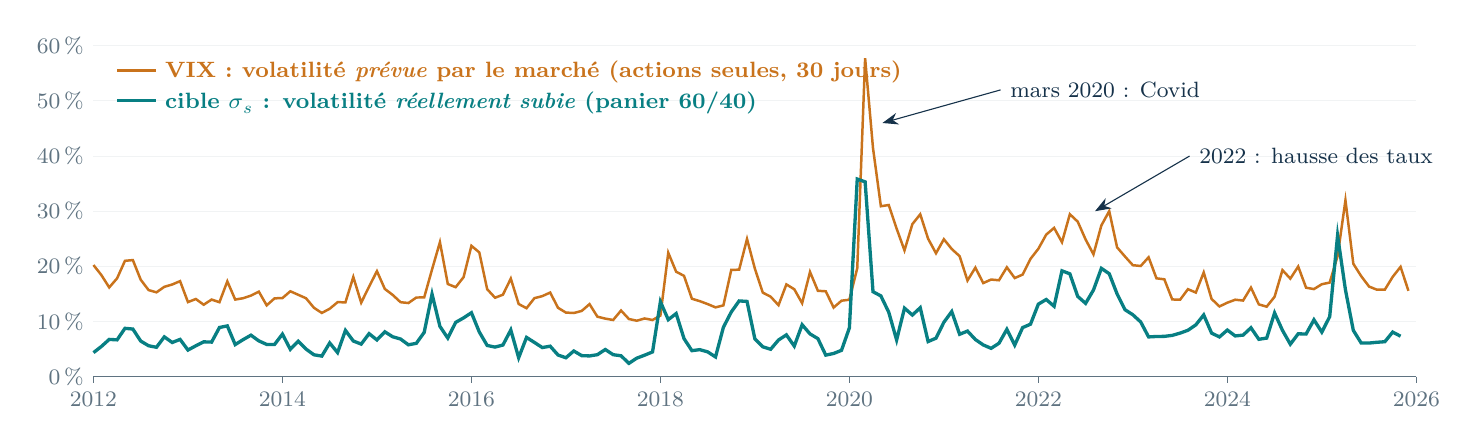
\begin{tikzpicture}[x=1.2cm,y=0.07cm,font=\footnotesize]
  \foreach \y in {0,10,...,60} {\draw[gris!70!discret!25] (0,\y) -- (14,\y); \node[left,text=discret] at (0,\y) {\y\,\%};}
  \foreach \a in {0,2,...,14} {\draw[discret] (\a,0) -- (\a,-1.2); \pgfmathtruncatemacro{\an}{2012+\a}\node[below,text=discret] at (\a,-1) {\an};}
  \draw[discret] (0,0) -- (14,0);
  \tracevix{orange,line width=0.9pt}
  \tracecible{sarcelle,line width=1.2pt}
  \node[anchor=north west,text=orange,font=\footnotesize\bfseries] at (0.15,59) {\rule[2pt]{14pt}{1pt}\ VIX : volatilité \emph{prévue} par le marché (actions seules, 30 jours)};
  \node[anchor=north west,text=sarcelle,font=\footnotesize\bfseries] at (0.15,53.5) {\rule[2pt]{14pt}{1.4pt}\ cible $\sigma_s$ : volatilité \emph{réellement subie} (panier 60/40)};
  \draw[marine,-{Stealth[length=2mm]}] (9.6,52) -- (8.35,46); \node[anchor=west,text=marine] at (9.6,52) {mars 2020 : Covid};
  \draw[marine,-{Stealth[length=2mm]}] (11.6,40) -- (10.6,30); \node[anchor=west,text=marine] at (11.6,40) {2022 : hausse des taux};
\end{tikzpicture}\\[-2pt]
{\footnotesize\color{discret}Figure 1 — Cible et VIX, moyennes mensuelles 2012–2025, en \% annuel (données de \fic{data/prepare/}, script \fic{docs/latex/generer\_figures.py}). Le jour même, le VIX vaut en médiane 2,3 fois la cible.}
\end{center}

\subsection{Indicateurs implicites B (surface, 2017–2023)}
\textbf{Ce que l'on veut.} Les variables B résument en 8 chiffres ce que \textbf{les prix des options sur le S\&P~500 disent du risque à venir} : le niveau de risque attendu (IV), le prix de la protection contre la baisse (skew) et l'inquiétude à court terme comparée au moyen terme (pente).

\textbf{Ce que l'on a.} Pour chaque jour de 2017 à 2023, la surface (section~\ref{sec:donnees}) est un tableau de volatilités implicites de \textbf{32 lignes} (prix d'exercice de 80\,\% à 120\,\% du cours, par pas d'environ 1,3\,\%) et \textbf{16 colonnes} (échéances de 7 à 365 jours, de plus en plus espacées : 7, 9, 12, 15, 20, 26, 34, 44, 58\,… jours).

\textbf{Le problème.} Les points qui nous intéressent (95\,\%, 100\,\% et 105\,\% du cours ; 30 et 60 jours) \textbf{ne sont pas dans le tableau}. Par exemple, 95\,\% tombe entre les lignes 94,2\,\% et 95,5\,\%, et 30 jours entre les colonnes 26 et 34 jours. On calcule donc la valeur entre deux cases voisines, en deux temps : d'abord entre deux prix d'exercice \eqref{eq:interpm}, puis entre deux échéances \eqref{eq:interpT}. Chaque jour est traité seul, sans aucune information d'un autre jour : aucune fuite du futur n'est possible.

\begin{formule}{Interpolation de la surface et indicateurs implicites}
\begin{equation}\label{eq:interpm}
\sigma^2(m^\star,T)=(1-\lambda)\,\sigma^2(m_1,T)+\lambda\,\sigma^2(m_2,T),\qquad \lambda=\frac{m^\star-m_1}{m_2-m_1}
\end{equation}
\begin{equation}\label{eq:interpT}
w(T)=\sigma^2(T)\,T,\qquad w(T^\star)=w(T_1)+\mu\,\bigl(w(T_2)-w(T_1)\bigr),\quad \mu=\frac{T^\star-T_1}{T_2-T_1},\qquad \sigma(T^\star)=\sqrt{w(T^\star)/T^\star}
\end{equation}
\begin{equation}\label{eq:skewpente}
\mathrm{skew}_{30}=\sigma(0{,}95;30)-\sigma(1;30),\qquad \mathrm{pente}_{60/30}=\sigma(1;60)-\sigma(1;30)
\end{equation}
\notation{$K,\ S$}{prix d'exercice de l'option et cours du S\&P~500 le jour de l'observation (\emph{spot})}
\notation{$m=K/S$}{\textbf{prix d'exercice relatif} (\emph{moneyness}) : 0,95 = 5\,\% sous le cours (put protecteur), 1 = au cours (à la monnaie), 1,05 = 5\,\% au-dessus}
\notation{$m^\star;\ m_1,m_2$}{niveau recherché (0,95, 1 ou 1,05) ; les deux lignes du tableau juste en dessous et juste au-dessus}
\notation{$\lambda$}{\textbf{poids} donné à la ligne du dessus, entre 0 et 1 : plus $m^\star$ est proche de $m_2$, plus $\lambda$ est proche de 1}
\notation{$T^\star;\ T_1,T_2;\ \mu$}{échéance recherchée (30 ou 60 jours calendaires) ; les deux colonnes qui l'encadrent ; poids donné à $T_2$, comme $\lambda$}
\notation{$\sigma(m;T)$}{\textbf{volatilité implicite} au niveau $m$ et à l'échéance $T$, en \% annuel}
\notation{$\sigma^2$}{on mélange les \textbf{carrés} des volatilités (des variances), pas les volatilités elles-mêmes : c'est la variance qui s'additionne proprement}
\notation{$w(T)$}{\textbf{variance totale} : IV au carré fois durée, c'est-à-dire le risque cumulé jusqu'à l'échéance. Le risque sur 34 jours contient celui sur 26 jours, donc $w$ doit croître avec $T$ : en interpolant $w$, on garde cette cohérence \cite{gatheral}}
\notation{$\mathrm{skew}_{30}$}{\textbf{asymétrie du sourire} à 30 jours, en points de volatilité : combien la protection contre une baisse de 5\,\% coûte de plus que l'option au cours}
\notation{$\mathrm{pente}_{60/30}$}{\textbf{pente de la structure par terme} au cours, en points : positive, le marché craint plus le moyen terme (normal) ; négative, il craint surtout les jours qui viennent (crise)}
\end{formule}

\textbf{Exemple du 1\textsuperscript{er} juillet 2022, calcul de $\sigma(0{,}95;30)$.}
\begin{enumerate}[nosep,leftmargin=*]
  \item \emph{Entre les deux prix d'exercice.} $m_1=94{,}19\,\%$ et $m_2=95{,}48\,\%$, donc $\lambda=(95-94{,}19)/(95{,}48-94{,}19)=0{,}625$. À 26 jours, les IV du tableau sont 28,26\,\% et 27,39\,\% : $\sigma^2=0{,}375\times28{,}26^2+0{,}625\times27{,}39^2$, soit $\sigma=27{,}72\,\%$. À 34 jours, de même : $27{,}67\,\%$.
  \item \emph{Entre les deux échéances.} $w(26{,}15)=27{,}72^2\times26{,}15=20\,095$ et $w(34{,}04)=27{,}67^2\times34{,}04=26\,066$. $\mu=(30-26{,}15)/(34{,}04-26{,}15)=0{,}488$, donc $w(30)=20\,095+0{,}488\times(26\,066-20\,095)=23\,009$ et $\sigma=\sqrt{23\,009/30}=\textbf{27,69\,\%}$.
  \item \emph{Indicateurs du jour.} L'IV au cours vaut 24,44\,\% : le skew vaut $27{,}69-24{,}44=\textbf{3,25 points}$. À 60 jours, l'IV au cours vaut 24,72\,\%, d'où une pente de \textbf{+0,28 point}. Le VIX du jour vaut 26,7.
\end{enumerate}

{\small
\begin{tabularx}{\linewidth}{@{}L{4.2cm} Y L{2.3cm}@{}}
\rowcolor{marine}\entete{Colonne} & \entete{Nom complet} & \entete{Formule} \\
\fic{iv\_30j\_95spot\_pct} & volatilité implicite à 30 jours, prix d'exercice à 95\,\% du cours (put protecteur) & $\sigma(0{,}95;30)$ \\
\rowcolor{gris}\fic{iv\_30j\_100spot\_pct} & volatilité implicite à 30 jours, à la monnaie & $\sigma(1;30)$ \\
\fic{iv\_30j\_105spot\_pct} & volatilité implicite à 30 jours, prix d'exercice à 105\,\% du cours & $\sigma(1{,}05;30)$ \\
\rowcolor{gris}\fic{iv\_60j\_\{95,100,105\}spot\_pct} & mêmes volatilités implicites, à 60 jours & $\sigma(m;60)$ \\
\fic{skew\_30j\_points} & asymétrie du sourire à 30 jours & \eqref{eq:skewpente} \\
\rowcolor{gris}\fic{pente\_60j\_30j\_points} & pente de la structure par terme à la monnaie & \eqref{eq:skewpente} \\
\end{tabularx}}

\textbf{Ce que disent les chiffres} (1\,734 séances complètes, 2017–2023, après le contrôle de qualité de la section~\ref{sec:controles}).
\begin{itemize}[nosep,leftmargin=*]
  \item \textbf{Skew} : 4,9 points en médiane, toujours positif (de 0,25 à 7,2). La protection contre la baisse coûte donc toujours plus cher que l'option au cours : c'est le « sourire en pente » typique des actions.
  \item \textbf{Pente} : 0,9 point en médiane. Elle est négative 13,7\,\% du temps, surtout en 2018, 2020 et 2022 (VIX moyen de 31 ces jours-là, contre 17 sinon), et descend jusqu'à $-9{,}1$ points le 12 mars 2020 : ce jour-là, le marché redoutait bien plus les 30 jours à venir que les 60.
  \item \textbf{VIX et IV au cours} : ils montent et baissent ensemble (corrélation des niveaux de 0,99), mais le VIX est en moyenne \textbf{3,6 points plus haut}. Le VIX mélange les options de tous les prix d'exercice \eqref{eq:vix}, y compris les puts éloignés, plus chers ; $\sigma(1;30)$ n'utilise que l'option au cours. Les deux ne sont donc pas interchangeables, et les garder tous les deux renseigne aussi sur le sourire.
  \item \textbf{Vérification} : j'ai recalculé trois de ces IV directement depuis le tableau brut, avec un programme écrit séparément. L'écart est inférieur à $10^{-5}$ point : le calcul est fiable.
\end{itemize}

\subsection{Ce qui n'est pas construit : la volatilité locale C}
La volatilité implicite donne \textbf{un risque moyen} jusqu'à une échéance. La \textbf{volatilité locale} va plus loin : elle dit quel risque le marché attend \emph{à une date précise} et \emph{si l'indice se trouve à un niveau précis} (par exemple : « dans 20 jours, si le S\&P~500 a baissé de 5\,\% »). On l'obtient à partir de la même surface, avec la formule de Dupire.
\begin{attention}{Formule de Dupire et pourquoi je ne l'ai pas encore construite}
\begin{equation}\label{eq:dupire}
\sigma^2_{\mathrm{loc}}(T,K)=\frac{\partial_T C+(r-q)\,K\,\partial_K C+q\,C}{\tfrac12\,K^2\,\partial^2_{KK}C}
\end{equation}
\notation{$\sigma_{\mathrm{loc}}(T,K)$}{\textbf{volatilité locale} : risque attendu à la date $T$ si l'indice vaut alors $K$}
\notation{$C(T,K)$}{prix, le jour de l'observation, d'un call européen d'échéance $T$ et de prix d'exercice $K$}
\notation{$\partial_T,\ \partial_K,\ \partial^2_{KK}$}{dérivées : de combien le prix du call change si l'on allonge un peu l'échéance ($\partial_T$), si l'on monte un peu le prix d'exercice ($\partial_K$), et comment ce changement varie lui-même ($\partial^2_{KK}$, dérivée seconde)}
\notation{$r,\ q$}{taux sans risque et rendement du dividende, supposés constants ici}
\textbf{Pourquoi c'est difficile.} La formule \cite{dupire} dérive les prix des options \emph{deux fois}. Or chaque dérivée grossit les erreurs : une petite erreur sur un prix devient une grosse erreur sur la volatilité locale. Il faut donc une surface très propre et sans arbitrage, en pratique un sourire SVI ajusté à chaque échéance \cite{gatheraljacquier}.

\textbf{Ce qu'il faut, ce que nous avons, ce qui manque.}

{\small
\begin{tabularx}{\linewidth}{@{}L{4.6cm} Y Y@{}}
\rowcolor{marine}\entete{Il faut} & \entete{Nous avons} & \entete{Il manque} \\
les prix bruts des options (achat et vente), pour beaucoup de prix d'exercice autour du cours & une surface déjà lissée et complétée par d'autres ; des prix bruts sur 6 mois (2022) & des prix bruts sur toute la période \\
\rowcolor{gris}un long historique, idéalement 2012–2025 & la surface sur 2017–2023 & 2012–2016 et 2024–2025 \\
le prix à terme de l'indice pour chaque échéance (il tient compte des taux et des dividendes) & estimé seulement sur l'échantillon 2022 & les prix à terme sur toute la période \\
\rowcolor{gris}l'heure de chaque prix, pour prendre options et indice au même moment & aucune heure & des données horodatées \\
une méthode stable : sourire SVI sans arbitrage, calcul des dérivées, rejet des jours instables & rien n'est codé & le code, faisable dès maintenant sur l'échantillon 2022 \\
\end{tabularx}}

Ce qui manque surtout, ce sont \textbf{les données}. Voici précisément ce qu'il faut demander (à Bloomberg, ou à défaut à OptionMetrics ou Cboe DataShop) :

{\small
\begin{tabularx}{\linewidth}{@{}L{3.2cm} Y@{}}
\rowcolor{marine}\entete{Donnée} & \entete{Détail précis} \\
Quelles options & options européennes sur l'indice S\&P~500 cotées au Cboe : SPX (mensuelles, réglées le matin, AM) et SPXW (hebdomadaires, réglées le soir, PM), en indiquant pour chaque option de quel type elle est \\
\rowcolor{gris}Quelle période & chaque séance de Bourse du 1\textsuperscript{er} août 2011 (période de démarrage des variables A) au 31 décembre 2025 \\
Quand dans la journée & \textbf{une photo par jour à heure fixe}, par exemple 15 h 45 à New York (un quart d'heure avant la clôture), avec le niveau du SPX \textbf{à la même minute}. Notre échantillon 2022 n'a pas d'heure : la colonne existe mais elle est vide \\
\rowcolor{gris}Pour chaque option & date et heure du prix ; SPX ou SPXW ; date d'échéance ; prix d'exercice ; call ou put ; \textbf{meilleur prix d'achat} (\emph{bid}) et \textbf{meilleur prix de vente} (\emph{ask}) ; volume du jour et nombre de contrats ouverts (\emph{open interest}), pour écarter les options trop peu échangées. L'IV calculée par le fournisseur est utile pour un contrôle, mais pas indispensable \\
Quels prix d'exercice, quelles échéances & au moins de 70\,\% à 130\,\% du cours, et de 7 jours à 1 an ; surtout, \textbf{calls et puts aux mêmes prix d'exercice} : la parité call-put en déduit alors, pour chaque échéance, le prix à terme et le facteur d'actualisation (méthode déjà codée sur 2022) \\
\rowcolor{gris}Taux et dividendes & la courbe des taux sans risque de 1 mois à 1 an, chaque jour (gratuite sur le site du Trésor américain), et si possible le rendement de dividende attendu du S\&P~500 : ils servent à vérifier les prix à terme tirés de la parité \\
\end{tabularx}}

Pour fixer l'ordre de grandeur : en 2022, une séance compte environ \textbf{19\,400 options} SPX et SPXW. Sur 2011–2025, cela fait plusieurs dizaines de millions de lignes, à prévoir dans un format compressé. Je conseille de ne construire C qu'une fois ces données obtenues. En attendant, on peut écrire et tester le code sur l'échantillon 2022.
\end{attention}

% ================================================================
\section{Exemple complet : le signal du 1\textsuperscript{er} juillet 2022}\label{sec:exemple}
Pour rendre chaque formule concrète, voici toutes les valeurs d'une même ligne, celle du vendredi 1\textsuperscript{er} juillet 2022. Chacune peut être recalculée à la main à partir des fichiers. Colonne de gauche : les marchés et les variables A ; colonne de droite : les indices Cboe, la surface (B), le cash et la cible.

{\small
\begin{tabularx}{\linewidth}{@{}Y r Y r@{}}
\rowcolor{marine}\entete{Donnée du 01/07/2022} & \entete{Valeur} & \entete{Donnée du 01/07/2022} & \entete{Valeur} \\
SPX, clôture & 3\,825,33 pts & VIX9D / VIX & 23,56 / 26,70 \\
\rowcolor{gris}SPY : cours coté / ajusté & 381,24 / 360,49 \$ & VIX3M / VIX6M & 28,52 / 29,93 \\
IEF : cours coté / ajusté & 103,24 / 89,08 \$ & SKEW & 118,59 \\
\rowcolor{gris}IEF : distribution détachée ce jour & 0,155 \$ & $\sigma(0{,}95;30)$ / $\sigma(1;30)$ / $\sigma(1{,}05;30)$ & 27,69 / 24,44 / 21,12 \\
$r_{\SPY}$ / $r_{\IEF}$ \eqref{eq:rendement} & +1,058\,\% / +1,072\,\% & $\sigma(0{,}95;60)$ / $\sigma(1;60)$ / $\sigma(1{,}05;60)$ & 27,67 / 24,72 / 21,55 \\
\rowcolor{gris}$q$ \eqref{eq:panier} & +1,063\,\% & skew$_{30}$ / pente$_{60/30}$ \eqref{eq:skewpente} & 3,25 / 0,28 pt \\
\fic{var\_panier\_5 / 21 / 63} & 0,0175 / 0,0410 / 0,0323 & cash \eqref{eq:cash} : T-bill publié le 30/06, $1{,}15\,\% \times 1/365$ & 0,0000315 \\
\rowcolor{gris}soit en volatilité & 13,2 / 20,2 / 18,0\,\% & RF de French & 0 \\
\fic{var\_spy\_21} / \fic{var\_ief\_21} & 0,0904 / 0,0165 & Hamidieh : skew / straddle & $-0{,}057$ / 0,184 \\
\rowcolor{gris}\fic{rend\_panier\_21 / 63} & $-3{,}59$ / $-10{,}46$\,\% & achat ($s+1$) & 05/07/2022 \\
\fic{semivar\_baisse\_21} & 0,0267 & fin de la cible ($s+22$) & 03/08/2022 \\
\rowcolor{gris}\fic{corr\_spy\_ief\_21 / 63} & +0,31 / +0,10 & \textbf{cible} $\sigma_s$ \eqref{eq:cible} & \textbf{12,93\,\%} \\
\end{tabularx}}

\textbf{Comment retrouver ces chiffres.}
\begin{itemize}[nosep,leftmargin=*]
  \item \textbf{Cours coté et cours ajusté} : le cours ajusté de SPY (360,49) est plus bas que le cours coté (381,24), car Yahoo abaisse les prix passés de tous les dividendes versés depuis. Seuls les rendements comptent, et ils sont identiques avec les deux.
  \item \textbf{Rendement d'IEF} : IEF détache 0,155~\$ ce jour-là. Le rendement compte le prix \emph{et} cette distribution : $(103{,}24+0{,}155)/102{,}30-1=+1{,}07\,\%$.
  \item \textbf{Panier} : $q=0{,}6\times1{,}058+0{,}4\times1{,}072=+1{,}063\,\%$.
  \item \textbf{Variances en volatilités} : on prend la racine carrée, par exemple $\sqrt{0{,}0410}=20{,}2\,\%$ sur 21 séances.
  \item \textbf{Corrélations positives} (+0,31 sur 21 séances) : en 2022, actions et obligations baissaient ensemble, et IEF ne protégeait plus le panier.
  \item \textbf{Cash} : le taux du T-bill publié la veille, 1,15\,\% par an, pour 1 jour : $1{,}15\,\%/365=0{,}00315\,\%$. Le RF de French, arrondi à 0,01\,\% par jour, tombe à 0.
  \item \textbf{Hamidieh} : skew de $-0{,}057$, soit des calls hors de la monnaie 5,7 points de volatilité moins chers que les puts ; straddle de 0,184, soit une volatilité d'environ $0{,}184/0{,}8\approx23\,\%$.
\end{itemize}

\textbf{Calcul de la cible pas à pas.}
\begin{enumerate}[nosep,leftmargin=*]
\item On achète le mardi 5 juillet, la séance qui suit le signal (le lundi 4 juillet est férié). Le panier y vaut $B=1$. Les jours suivants, il vaut 0,998629, puis 1,005214, puis 1,002318, et il finit à 1,055411 le 3 août.
\item Les rendements $b$ valent $-0{,}137\,\%$, $+0{,}659\,\%$, $-0{,}288\,\%$, etc. La somme de leurs 21 carrés vaut 0,0013939.
\item D'où $y_s=\frac{252}{21}\times0{,}0013939=0{,}016727$ et $\sigma_s=\sqrt{0{,}016727}=12{,}93\,\%$.
\end{enumerate}

\textbf{Ce que cet exemple apprend.} Ce jour-là, la volatilité des 21 dernières séances était de 20,2\,\% et le VIX valait 26,7. Le risque réellement subi ensuite n'a été que de \textbf{12,9\,\%}. Le marché venait de traverser un mois de juin très agité, puis il s'est calmé en juillet. Voici ce que cela change pour la règle d'allocation \eqref{eq:allocation} :
\begin{itemize}[nosep,leftmargin=*]
  \item prévoir avec la volatilité passée (20,2\,\%) aurait fait investir $8/20{,}2=40\,\%$ ;
  \item prévoir avec le VIX (26,7\,\%) aurait fait investir $8/26{,}7=30\,\%$ ;
  \item la bonne réponse (12,93\,\%) aurait fait investir $8/12{,}93=62\,\%$.
\end{itemize}
Un bon modèle doit donc comprendre que le risque d'hier ne dure pas toujours, et que le VIX surestime le risque du panier. C'est exactement ce que les ensembles A, B et C doivent apprendre.

% ================================================================
\section{Contrôles de qualité et corrections}\label{sec:controles}
Une donnée fausse donne un modèle faux, même s'il est bien construit. J'ai donc vérifié chaque source par une autre source indépendante. Cette section décrit ce que j'ai trouvé et ce que j'ai corrigé.

\subsection{Six surfaces corrompues en mai 2019}
\textbf{Comment je l'ai vu.} Le VIX, calculé par Cboe à partir des mêmes options, sert de témoin : il doit bouger presque comme l'IV au cours $\sigma(1;30)$. Chaque année, la corrélation de leurs variations d'un jour à l'autre dépasse 0,93. En 2019, elle tombait à 0,46. La cause : six grilles fausses, avec un sourire plat et une IV qui monte jusqu'à 60\,\% à un an.

\begin{minipage}[t]{0.5\linewidth}\vspace{0pt}
{\small
\begin{tabular}{@{}l r r r r@{}}
\rowcolor{marine}\entete{Séance} & \entete{VIX} & \entete{$\sigma(1;30)$} & \entete{écart} & \entete{pente 90/100} \\
02/05/2019 & 14,42 & 27,84 & \textcolor{rouge}{+13,42} & 0,37 \\
\rowcolor{gris}03/05/2019 & 12,87 & 27,57 & \textcolor{rouge}{+14,70} & 0,00 \\
06/05/2019 & 15,44 & 28,31 & \textcolor{rouge}{+12,87} & $-0{,}38$ \\
\rowcolor{gris}07/05/2019 & 19,32 & 30,70 & \textcolor{rouge}{+11,38} & 0,76 \\
08/05/2019 & 19,40 & 31,04 & \textcolor{rouge}{+11,64} & 0,24 \\
\rowcolor{gris}17/05/2019 & 15,96 & 30,55 & \textcolor{rouge}{+14,59} & $-0{,}69$ \\
\end{tabular}}
\end{minipage}\hfill
\begin{minipage}[t]{0.47\linewidth}\vspace{0pt}
\begin{correction}{Règle de rejet}
\begin{equation}\label{eq:rejet}
\begin{gathered}
\sigma_t(1;30)-\mathrm{VIX}_t>5\\[-1pt]
\text{ou}\\[-1pt]
\sigma_t(0{,}9;30)-\sigma_t(1;30)<2
\end{gathered}
\end{equation}
En points de volatilité, à la même clôture. Les deux critères isolent \textbf{les mêmes six séances}.
\end{correction}
\end{minipage}

\textbf{La règle en clair.} Une surface est rejetée dans deux cas :
\begin{itemize}[nosep,leftmargin=*]
  \item \emph{l'IV au cours dépasse le VIX de plus de 5 points}. Normalement, c'est l'inverse : le VIX inclut les puts éloignés, plus chers, et il est au-dessus de l'IV au cours \textbf{tous les jours} restants, d'au moins 0,85 point ;
  \item \emph{le sourire est plat} : un put 10\,\% sous le cours coûte moins de 2 points de volatilité de plus que l'option au cours. Sur les actions, la protection contre la baisse coûte toujours plus cher. Les autres jours, cet écart vaut au moins 3,07 points.
\end{itemize}
Les seuils de 5 et de 2 points sont loin des valeurs normales : la règle ne rejette aucun bon jour par erreur.

\textbf{La correction.} Les huit colonnes de surface de ces six dates sont \textbf{vidées, sans remplissage} (on n'invente pas de valeur). Il reste 1\,734 séances. Après correction, la corrélation par année vaut, de 2017 à 2023 : 0,94 ; 0,93 ; \textbf{0,96} ; 0,97 ; 0,96 ; 0,94 ; 0,95. Le détail par date est dans \fic{controles/controle\_qualite\_surface.csv}.

\subsection{Autres anomalies de la surface}
\begin{itemize}
\item \textbf{Dix dates où la Bourse est fermée} (fêtes de 2022, et le 5 décembre 2018, jour de deuil national pour le président Bush). La surface y contient des valeurs, mais ce ne sont ni celles de la veille ni la moyenne de la veille et du lendemain. Je les écarte. J'ai aussi vérifié que les dates ne sont pas décalées d'un jour : avec la veille ou le lendemain, la corrélation avec le VIX tombe près de 0 chaque année.
\item \textbf{Trois IV à 7 jours valent 0,00072\,\%} le 16 juin 2017, un jour d'échéance mensuelle. C'est sans doute un effet du prolongement de la surface par ses auteurs (section~\ref{sec:fournisseurs}). Elles n'affectent pas les indicateurs à 30 et 60 jours. La colonne \fic{cellules\_sous\_1pct} les compte.
\end{itemize}

\subsection{VIX9D et VIX6M reconstruits après coup}
Cboe a lancé le VIX9D le 1\textsuperscript{er} octobre 2013 et le VIX6M le 27 novembre 2013 \cite{cboe9d,cboe6m}. Le fichier contient pourtant des valeurs plus anciennes : Cboe les a recalculées plus tard. Personne ne pouvait donc les lire à l'époque, et un modèle qui les utilise avant cette date triche sans le savoir. La colonne \fic{vix9d\_vix6m\_diffuses} vaut \emph{vrai} à partir du 27/11/2013 : un backtest qui utilise ces deux séries doit se limiter à ces lignes. Le VIX et le VIX3M sont utilisables dès 2012.

\subsection{Contrôle de la surface par les vrais contrats de 2022}
La surface a été lissée et complétée par ses auteurs. Je l'ai donc comparée aux \textbf{vrais prix des options} de l'échantillon OptionsDX du second semestre 2022.

\textbf{Filtre de qualité.} Un prix est utilisable (colonne \fic{quality\_ok}) si toutes ces conditions sont réunies :
\begin{itemize}[nosep]
\item l'IV est positive et le fournisseur l'a calculée sans anomalie (colonne \fic{iv\_flag} égale à 0) ;
\item le prix d'achat (bid) est strictement positif et le prix de vente (ask) lui est au moins égal ;
\item l'échéance n'est pas encore passée ;
\item l'option est européenne, réglée le matin (AM) ou le soir (PM).
\end{itemize}
C'est le cas de 86,6\,\% des lignes, soit 2\,149\,547.

\begin{formule}{IV au cours recalculée depuis les contrats}
\begin{equation}\label{eq:ivspot}
\sigma(1,T)=\sigma(m_1,T)+\frac{1-m_1}{m_2-m_1}\bigl(\sigma(m_2,T)-\sigma(m_1,T)\bigr)
\end{equation}
\notation{$m_1\le1\le m_2$}{prix d'exercice relatifs des deux contrats juste sous et juste au-dessus du cours, entre 0,97 et 1,03}
\notation{$\sigma(m,T)$}{IV donnée par le fournisseur, pour les options PM de 15 à 50 jours : puts sous le cours, calls au-dessus, car ce sont les plus échangés (médiane si plusieurs contrats)}
On ramène ensuite l'IV à 30 jours par la variance totale \eqref{eq:interpT}, comme pour la surface.
\end{formule}
\textbf{Résultat.} Sur 126 séances communes, l'écart entre la surface et les vrais contrats vaut \textbf{0,55 point} en médiane, et moins de \textbf{1,31 point} dans 95\,\% des cas. Pour une IV d'environ 25\,\% en 2022, c'est une erreur d'environ 2\,\% de sa valeur : le centre de la surface est fiable.

\begin{attention}{Biais de niveau}
En moyenne, la surface est \textbf{0,50 point plus basse} que les vrais contrats. C'est peu gênant pour un modèle qui apprend des variations, mais il faut le signaler. Attention : seul le centre de la surface (autour du cours) est vérifié, et seulement en 2022.
\end{attention}

\textbf{Prix à terme : un travail préparé pour C.} Pour la volatilité locale, il faudra le prix à terme $F$ de l'indice à chaque échéance. On peut le tirer des prix des options grâce à la \textbf{parité call-put} : un call acheté et un put vendu au même prix d'exercice reviennent à acheter l'indice à terme.
\begin{formule}{Prix à terme par la parité call-put \cite{hull}}
\begin{equation}\label{eq:parite}
C-P=D(T)\,(F-K)\ \Rightarrow\ F=K+\frac{C-P}{D(T)},\qquad D(T)=1-\frac{d}{100}\,\frac{T}{360}
\end{equation}
\begin{equation}\label{eq:bornes}
F^{\mathrm{bas}}=K+\frac{C^{\mathrm{bid}}-P^{\mathrm{ask}}}{D(T)},\qquad F^{\mathrm{haut}}=K+\frac{C^{\mathrm{ask}}-P^{\mathrm{bid}}}{D(T)},\qquad \ln D(T)=(1-\lambda)\ln D(T_1)+\lambda\ln D(T_2)
\end{equation}
\notation{$C,\ P$}{prix d'un call et d'un put européens de même échéance $T$ et de même prix d'exercice $K$}
\notation{$C^{\mathrm{bid}},C^{\mathrm{ask}}$}{prix auxquels on peut vendre (bid) et acheter (ask) le call sur le marché ; de même pour le put}
\notation{$D(T)$}{\textbf{facteur d'actualisation} : ce que vaut aujourd'hui 1~\$ reçu à l'échéance $T$, tiré du T-bill \eqref{eq:tbill}}
\notation{$T_1,T_2,\lambda$}{échéances de T-bills qui encadrent $T$, et poids d'interpolation}
\notation{$F;\ F^{\mathrm{bas}},F^{\mathrm{haut}}$}{\textbf{prix à terme} du SPX, et sa fourchette : le prix le plus bas et le plus haut compatibles avec les prix d'achat et de vente. On garde la médiane des milieux $(F^{\mathrm{bas}}+F^{\mathrm{haut}})/2$}
\end{formule}
J'utilise les options SPXW PM de 15 à 95 jours, entre 98 et 102\,\% du cours, avec au moins 3 paires call-put par échéance. On obtient 2\,102 estimations, avec 30 paires par échéance en médiane. La fourchette de $F$ mesure 1,26 point d'indice en médiane (0,03\,\% d'un indice vers 3\,900), et les estimations des différentes paires ne diffèrent que d'environ 0,05 point (écart interquartile médian). Le prix à terme reste toujours à moins de 1,04\,\% du cours. La méthode fonctionne : elle pourra servir telle quelle pour C.

\subsection{Audit indépendant}
\begin{valide}{48 contrôles sur 48 satisfaits — \fic{tests/audit\_donnees.py}}
Ce second programme n'utilise pas le code du projet : il relit lui-même les fichiers et recalcule chaque grandeur par un autre chemin. Si les deux programmes donnent le même résultat, une erreur de code est très peu probable. Il vérifie :
\begin{itemize}
\item les fichiers bruts, le calendrier, des prix toujours positifs et la cohérence entre SPX et SPY (corrélation des rendements de 0,9986, car SPY réplique le S\&P~500) ;
\item les 13 variables A, recalculées autrement (écart maximal de $1{,}7\times10^{-10}$) ;
\item l'absence de fuite du futur : si l'on modifie les rendements futurs, aucune variable passée ne change ;
\item la cible, recalculée par une boucle simple à partir des prix Yahoo bruts (écart relatif maximal de $4{,}9\times10^{-10}$, la précision d'un fichier à 10 chiffres) ;
\item les bornes des indices, la forme du sourire, l'IV sous le VIX chaque jour, le cash, le contrôle de la surface et les prix à terme.
\end{itemize}
\end{valide}

% ================================================================
\section{Hypothèses du travail}\label{sec:hypotheses}
Une hypothèse est un choix que j'ai fait sans pouvoir le prouver totalement. Pour chacune, j'indique ce qu'elle veut dire, pourquoi elle est raisonnable et ce qu'il faut surveiller.

{\small
\begin{longtable}{@{}>{\leavevmode\bfseries\color{sarcelle}}p{0.65cm} L{7.4cm} L{9.1cm}@{}}
\rowcolor{marine} & \entete{Hypothèse, en clair} & \entete{Pourquoi elle est raisonnable, ce qu'il faut surveiller} \\
\endhead
H1 & Toutes les séries suivent les jours d'ouverture de la Bourse de New York (NYSE). Un jour sans donnée reste vide : je n'invente aucune valeur. & On voit les trous au lieu de les cacher. Les modèles devront décider quoi en faire (ignorer la ligne, ou utiliser seulement A). \\
\rowcolor{gris}H2 & Les cours ajustés de Yahoo tiennent correctement compte des dividendes \eqref{eq:ajustement}. & Je retrouve les rendements de Yahoo à 0,02~pb près, et les 56 dividendes de SPY et 168 distributions d'IEF correspondent à ceux publiés par les émetteurs. \\
H3 & Pour les variables A, le panier est remis à 60/40 chaque jour \eqref{eq:panier}. & C'est une approximation commode pour décrire le passé. La cible, elle, suit le vrai panier, dont les poids bougent avec les prix \eqref{eq:valeurpanier}. \\
\rowcolor{gris}H4 & Une année compte 252 séances, et 21 séances font environ un mois. & C'est la convention de marché. Attention : les options comptent en jours calendaires, et 30 jours calendaires ne font pas exactement 21 séances. \\
H5 & Les variables A retirent la moyenne des rendements avant de les mettre au carré ; la cible ne le fait pas. & La moyenne quotidienne vaut environ 0,04\,\% : l'écart est négligeable (section~\ref{sec:variables}). \\
\rowcolor{gris}H6 & Le signal est calculé après la clôture du jour $s$ (16\,h\,15 à New York, fin de cotation des options SPX), et l'on achète à la clôture du lendemain $s+1$. & Le modèle n'utilise que des informations déjà connues, et laisser un jour pour agir est réaliste. \\
H7 & Le risque se mesure avec les prix de clôture, d'un jour au suivant, sans les mouvements à l'intérieur de la journée. & La cible est donc un peu « bruitée » (une journée agitée qui finit à plat compte peu). C'est pour cela que l'on juge les modèles avec QLIKE, qui supporte ce bruit \cite{patton}. \\
\rowcolor{gris}H8 & Le prix d'exercice est rapporté au cours du jour ($K/S$), et non au prix à terme ($K/F$). & À 30–60 jours, $F$ et $S$ diffèrent de moins de 1,04\,\% (mesuré sur 2022). C'est aussi la convention des auteurs de la surface. \\
H9 & Les auteurs de la surface lissent chaque jour avec les seules données de ce jour. & Leur code traite bien chaque jour séparément, et l'accord avec le VIX est vérifié chaque année. Sinon, la surface ferait fuiter le futur. \\
\rowcolor{gris}H10 & Le cash rapporte le taux du T-bill à 4 semaines publié la veille \eqref{eq:cash}. & Ce taux est connu au moment de décider et proche de ce que rapporte vraiment un placement sans risque. Il remplace le RF de French, trop arrondi. \\
H11 & Dans l'échantillon 2022, le call et le put sont cotés au même instant, et le jour de cotation est le jour de valeur. & Impossible à vérifier sans l'heure de cotation. Ces résultats servent donc de vérification, pas de donnée pour les modèles. \\
\end{longtable}}

% ================================================================
\section{Limites et points ouverts}
Ces limites ne bloquent pas le projet, mais il faut les connaître et savoir les dire à l'oral.
\begin{itemize}
\item \textbf{La surface couvre une période courte} : 1\,734 séances, de 2017 à 2023 seulement. Un modèle « A + surface » ne peut donc pas apprendre sur 2012–2016. Sur toute la période 2012–2025, l'information des options passe par les indices Cboe (VIX, VIX9D, VIX3M, VIX6M, SKEW).
\item \textbf{La surface n'est pas une donnée brute} : ses auteurs l'ont lissée (SVI), prolongée aux bords et complétée. Elle est fiable au centre (section~\ref{sec:controles}), moins sûre aux extrémités.
\item \textbf{On ne connaît pas l'heure exacte des prix}. Les variables de Hamidieh sont probablement relevées à 15\,h\,45 ; le VIX et les ETF ferment à des minutes un peu différentes. L'écart est faible d'un jour à l'autre, mais il existe.
\item \textbf{Les variables de Hamidieh} sont des moyennes sur des échéances qui changent chaque jour : je les garde pour vérifier, pas comme variables du modèle.
\item \textbf{Les données ont été téléchargées le 19 novembre 2026} : elles ont pu être corrigées depuis les dates qu'elles décrivent (par exemple, les cours ajustés de Yahoo changent à chaque nouveau dividende). Ce sont donc les données d'aujourd'hui, pas celles que l'on voyait à l'époque.
\item \textbf{La demande Bloomberg reste ouverte} (terminal de données financières, accessible par un contact à l'ESCP) : une grille 2012–2025 avec prix à terme, heure de cotation et façon de repérer les prix d'exercice ($K/S$, $K/F$ ou delta). Elle seule permettrait de construire C (section~\ref{sec:variables}).
\end{itemize}

% ================================================================
\section{Ce que je vous transmets et la suite}\label{sec:suite}
\subsection{Ce que vous avez entre les mains}
\textbf{Le dépôt GitHub du groupe}, copie (\emph{fork}) du dépôt du cours : \url{https://github.com/Cherif-D/ai_in_finance_volatilite_allocation}. Il contient le code, ce document (\fic{docs/}), les données préparées (\fic{data/prepare/*.csv}) et les contrôles. Le \fic{README.md} décrit le projet selon le modèle des enseignants. Pour le récupérer et vérifier que tout fonctionne (Windows, Python 3.12) :
\begin{verbatim}
git clone https://github.com/Cherif-D/ai_in_finance_volatilite_allocation.git
cd ai_in_finance_volatilite_allocation
py -3.12 -m venv .venv
.\.venv\Scripts\python.exe -m pip install -r requirements.txt
.\.venv\Scripts\python.exe -m unittest discover -s tests -v
\end{verbatim}
Les données brutes (247 Mo) et les deux fichiers tirés de l'échantillon d'options 2022 ne sont pas dans le dépôt, qui est public : \fic{scripts/01\_collecte.py} et \fic{03\_controle\_surface.py} les recréent si besoin (fichier \fic{DONNEES.md}).

\textbf{Les trois fichiers à utiliser}, dans \fic{data/prepare/} :
\begin{itemize}[nosep]
\item \fic{donnees\_quotidiennes.csv}, 29 colonnes : marchés, indices Cboe, surface, cash ;
\item \fic{variables\_A.csv}, les 13 variables, \textbf{connues} à la date de la ligne ;
\item \fic{cibles\_futures.csv}, la cible, \textbf{inconnue} à la date de la ligne.
\end{itemize}
Chaque colonne a sa fiche dans l'annexe~\ref{sec:fiches}. Le code qui les produit est dans \fic{portefeuille/} et \fic{scripts/}. Les tests et l'audit passent.

\begin{tcolorbox}[enhanced,breakable,colback=marine!4,colframe=marine!25,boxrule=0.5pt,arc=2pt,left=6pt,top=2pt,bottom=2pt,fontupper=\footnotesize,
  title={\faIcon{code}\enspace Exemple testé : charger les données, construire « A + indices Cboe », découper avec purge},fonttitle=\small\bfseries,coltitle=marine,colbacktitle=marine!4,titlerule=0pt,bottomtitle=0pt]
\begin{verbatim}
import numpy as np
import pandas as pd

def lire(nom):
    return pd.read_csv(f"data/prepare/{nom}", index_col="date", parse_dates=True)

quotidien, A, cible = lire("donnees_quotidiennes.csv"), lire("variables_A.csv"), lire("cibles_futures.csv")

# Ensemble « A + indices Cboe », à partir du 27/11/2013 (VIX9D et VIX6M publiés en temps réel)
X = A.join(quotidien[["vix9d", "vix", "vix3m", "vix6m", "skew"]])
X = X[quotidien["vix9d_vix6m_diffuses"]]
y = np.log(cible["variance_21j_ann"]).rename("log_variance")   # cible en logarithme
donnees = X.join(y).dropna()

# Découpage chronologique avec purge : test à partir du 01/01/2020 ;
# un exemple d'apprentissage doit avoir sa cible entièrement terminée avant le test.
debut_test = pd.Timestamp("2020-01-01")
fin_cible = pd.to_datetime(cible["fin_cible"]).reindex(donnees.index)
apprentissage = donnees[fin_cible < debut_test]
test = donnees[donnees.index >= debut_test]
# Résultat : 1508 exemples d'apprentissage (le dernier date du 27/11/2019), 1485 de test.
\end{verbatim}
\end{tcolorbox}
La purge se voit dans le résultat : les signaux de décembre 2019 sont écartés de l'apprentissage, car leur mois futur tombe en 2020, dans la période de test.

\subsection{Ce que le professeur attend}
D'après les consignes du cours \cite{cours6} :
\begin{itemize}[nosep]
\item \textbf{date limite : le 6 décembre 2026} (« 6/12 » dans les consignes) ;
\item \textbf{des diapositives, 10 au maximum}, pour un exposé de 8 à 10 minutes suivi de 3 à 5 minutes de questions. \textbf{Chaque membre du groupe présente une partie} ;
\item \textbf{le code}, en notebooks (\fic{.ipynb}) et en scripts (\fic{.py}), le mélange des deux étant encouragé, déposé dans une copie (\emph{fork}) du dépôt GitHub de base, partagée avec les enseignants. C'est le cas de notre dépôt (lien ci-dessus) : les notebooks vont dans \fic{notebooks/} (exploration) et \fic{selected\_approach/} (modèle retenu), les diapositives dans \fic{docs/} ;
\item \textbf{savoir défendre chaque choix} : l'IA est permise, mais chacun doit comprendre le code et pouvoir expliquer pourquoi on a fait ainsi. Ce document sert aussi à cela.
\end{itemize}

\subsection{La feuille de route, étape par étape}
Le cours recommande sept étapes \cite{cours6}. Les étapes 1, 3 et une grande partie de la 4 sont faites. Voici ce qu'il reste à faire, et à quoi s'attendre.

{\small
\begin{longtable}{@{}>{\leavevmode\bfseries\color{sarcelle}}p{2.1cm} L{7.6cm} L{7.2cm}@{}}
\rowcolor{marine}\entete{Étape} & \entete{Ce qu'il faut faire} & \entete{À quoi s'attendre} \\
\endhead
1. Problème & \textcolor{vert}{Fait} (section~\ref{sec:probleme}) : prévoir $\sigma_s$, puis investir $a=\min(1,\,8\,\%/\widehat\sigma)$. & Une diapositive : la question, la règle, les ensembles A, B, C. \\
\rowcolor{gris}2. Exploration & Un notebook : \texttt{describe()}, \texttt{info()}, histogrammes, carte des corrélations (\texttt{heatmap}), valeurs manquantes, graphe des crises 2020 et 2022. & La cible est très asymétrique : son logarithme l'est beaucoup moins. Les variances A sont très corrélées entre elles. Les manques sont tous expliqués (surface hors 2017–2023, VIX9D/VIX6M avant 2013, 22 dernières cibles). \\
3. Préparation & \textcolor{vert}{Fait} pour les données. Reste : le découpage dans le temps avec purge (exemple ci-dessus), et la mise à l'échelle des variables calculée \textbf{sur l'apprentissage seulement}. & Pas de \texttt{train\_test\_split} au hasard, contrairement à l'exemple du cours : les cibles se chevauchent sur 21 séances, et le hasard mélangerait passé et futur \cite{lopezdeprado}. \\
\rowcolor{gris}4. Variables & \textcolor{vert}{Fait} pour A et B. On peut ajouter, avec le passé seulement : le logarithme des variances, le rapport VIX / volatilité passée, l'écart VIX3M $-$ VIX. & Ces transformations aident surtout le modèle linéaire (Ridge). Les arbres en ont moins besoin. \\
5. Modèles & D'abord des \textbf{références simples} : persistance (volatilité des 21 dernières séances), EWMA \cite{riskmetrics}, GARCH(1,1) \cite{bollerslev}. Ensuite Ridge, forêt aléatoire et XGBoost sur $\log y_s$, avec A, puis A + indices Cboe, puis A + surface (2017–2023). Réglages choisis par validation glissante sur 2015–2019. & Battre la persistance et l'EWMA n'est pas garanti : ce sont de bonnes références. Avec environ 1\,500 exemples, Ridge fait souvent aussi bien que les arbres. Pour A + surface, l'échantillon est plus court : par exemple apprentissage 2017–2020, test 2021–2023. \\
\rowcolor{gris}6. Évaluation & MAE, RMSE, QLIKE \eqref{eq:metriques} et $R^2$ sur la période de test, \textbf{ensemble par ensemble} (A, A + Cboe, A + surface). Puis le backtest de la règle d'allocation. & Les erreurs se concentrent sur 2020 et 2022 : présenter les scores aussi hors de ces crises. Le premier indice (fin de section) laisse penser que les options aident. \\
7. Interprétation & Importance des variables, valeurs SHAP, coefficients de Ridge, et lecture économique. & Le VIX devrait compter, avec un effet inférieur à 1 pour 1 (il contient une prime de risque). La corrélation SPY-IEF devrait compter en 2022. \\
\end{longtable}}

\textbf{Les scores de l'étape 6.} Avec $\hat h_t$ la variance prévue, $y_t$ la variance réalisée et $n$ le nombre de dates de test :
\begin{equation}\label{eq:metriques}
\mathrm{MAE}=\frac1n\sum_t\bigl|\sqrt{\hat h_t}-\sqrt{y_t}\bigr|,\qquad
\mathrm{RMSE}=\sqrt{\frac1n\sum_t\bigl(\sqrt{\hat h_t}-\sqrt{y_t}\bigr)^2},\qquad
\mathrm{QLIKE}=\frac1n\sum_t\Bigl(\log\hat h_t+\frac{y_t}{\hat h_t}\Bigr)
\end{equation}
MAE et RMSE mesurent l'erreur moyenne sur la volatilité ; la RMSE punit davantage les grosses erreurs. QLIKE juge la variance : elle reste fiable même si la cible est mesurée avec du bruit \cite{patton}, et elle punit davantage une sous-estimation du risque qu'une surestimation. Pour tous ces scores, plus c'est bas, mieux c'est. Les modèles s'entraînent sur $\log y_s$ : il faut repasser à la variance ($\hat h=e^{\text{prévision}}$) avant de calculer les scores.

\textbf{Le backtest.} On applique la règle \eqref{eq:allocation} chaque jour sur la période de test : achat en $s+1$, 5~pb de frais à chaque changement de part investie, le reste placé au cash \eqref{eq:cash}. On compare à un panier 60/40 toujours investi à 100\,\%. Trois chiffres à présenter :
\begin{itemize}[nosep]
\item la \textbf{volatilité réalisée de la stratégie} : si les prévisions sont bonnes, elle doit être proche de l'objectif de 8\,\% ;
\item le \textbf{ratio de Sharpe} : rendement au-dessus du cash, divisé par la volatilité ;
\item la \textbf{perte maximale} (\emph{maximum drawdown}) : la plus forte baisse depuis un sommet.
\end{itemize}
Il ne faut pas promettre un meilleur rendement : l'intérêt des portefeuilles pilotés par la volatilité est débattu \cite{moreira,cederburg}. Le résultat attendu est surtout \textbf{un risque plus stable et des pertes plus faibles en crise}.

\textbf{Premier indice, à confirmer hors échantillon.} La cible est plus corrélée aux mesures tirées des options qu'à la volatilité passée sur 21 séances :
\begin{itemize}[nosep]
\item sur 2012–2025 (3\,498 dates) : 0,61 avec le VIX, contre 0,53 avec la volatilité passée ;
\item sur 2017–2023, la période de la surface (1\,734 dates) : 0,66 avec $\sigma(1;30)$ et 0,64 avec le VIX, contre 0,58 avec la volatilité passée.
\end{itemize}
Ces corrélations portent sur tout l'échantillon : ce ne sont pas des prévisions. Elles suggèrent que les options apportent de l'information, et c'est exactement ce que la suite doit prouver proprement.

\begin{retenir}{Plan proposé pour les deux semaines qui restent}
\begin{itemize}[leftmargin=1.2em,nosep]
\item \textbf{Du 23 au 29 novembre} : exploration (étape 2), découpage avec purge, références simples (persistance, EWMA, GARCH) et leurs scores. Répartir dès maintenant qui présente quelle partie.
\item \textbf{Du 30 novembre au 6 décembre} : Ridge, forêt aléatoire, XGBoost sur A, A + Cboe, A + surface ; scores, backtest, interprétation ; diapositives et répétition chronométrée.
\item \textbf{Les 10 diapositives}, selon la structure du cours : 1. le problème ; 2. les données (ce document, en une page) ; 3. l'exploration ; 4. les variables A, B, C ; 5. les modèles et le découpage avec purge ; 6. les scores ; 7. les résultats et le backtest ; 8. ce qui a marché ou non ; 9. la conclusion ; 10. le titre, ou un résultat de plus.
\end{itemize}
\end{retenir}

% ================================================================
\section{Annexe A : fiches de toutes les colonnes}\label{sec:fiches}
Valeurs typiques sur 2012–2025 : médiane, avec entre crochets les quantiles à 5\,\% et 95\,\%. Pour les variances, je donne la volatilité équivalente $\sqrt{v}$, plus parlante.

\subsection{\fic{donnees\_quotidiennes.csv} : une ligne par séance (3\,520 lignes)}
{\small
\begin{longtable}{@{}L{3.55cm} L{8.1cm} L{2.0cm} L{3.05cm}@{}}
\rowcolor{marine}\entete{Colonne} & \entete{Nom complet et calcul} & \entete{Unité ; source} & \entete{Valeurs typiques} \\
\endhead
\fic{spy\_close} & cours de clôture coté de SPY, $P_u$ & \$ ; Yahoo & 279 [141 ; 599] \\
\rowcolor{gris}\fic{spy\_adj} & cours de clôture ajusté de SPY, $P^{adj}_u$ \eqref{eq:ajustement} & \$ ; Yahoo & 249 [111 ; 588] \\
\fic{spy\_distribution} & dividende trimestriel détaché, $D_u$ (0 sinon) & \$ ; Yahoo & 56 jours non nuls ; max 1,99 \\
\rowcolor{gris}\fic{spy\_return} & rendement total quotidien de SPY, $r_u$ \eqref{eq:rendement} & décimal & 0,07\,\% [$-1{,}58$ ; 1,50\,\%] ; min $-10{,}9\,\%$ (16/03/2020) \\
\fic{spy\_ecart\_controle\_bp} & écart de contrôle $e_u$ \eqref{eq:controle} & pb & $\approx0$ ; max 2,52 \\
\rowcolor{gris}\fic{ief\_close}, \fic{ief\_adj} & cours coté et ajusté d'IEF & \$ ; Yahoo & 105 [94 ; 120] ; 85 [76 ; 102] \\
\fic{ief\_distribution} & coupon mensuel détaché & \$ ; Yahoo & 168 jours non nuls ; max 0,31 \\
\rowcolor{gris}\fic{ief\_return} & rendement total quotidien d'IEF & décimal & 0,02\,\% [$-0{,}64$ ; 0,62\,\%] \\
\fic{ief\_ecart\_controle\_bp} & écart de contrôle d'IEF & pb & $\approx0$ ; max 0,37 \\
\rowcolor{gris}\fic{spx\_close} & clôture de l'indice S\&P~500 & points ; Yahoo & 2\,798 [1\,409 ; 6\,006] \\
\fic{vix9d} & indice de volatilité de Cboe à 9 jours \eqref{eq:vix} & \% ; Cboe & 14,9 [9,7 ; 30,3] ; max 106,7 \\
\rowcolor{gris}\fic{vix} & indice de volatilité de Cboe à 30 jours \eqref{eq:vix30} & \% ; Cboe & 16,1 [11,2 ; 29,4] ; max 82,7 \\
\fic{vix3m} & indice de volatilité de Cboe à 3 mois & \% ; Cboe & 18,1 [13,4 ; 30,8] \\
\rowcolor{gris}\fic{vix6m} & indice de volatilité de Cboe à 6 mois & \% ; Cboe & 19,6 [15,2 ; 31,5] \\
\fic{skew} & indice d'asymétrie de Cboe \eqref{eq:skewcboe} & points ; Cboe & 130,6 [116,2 ; 154,1] \\
\rowcolor{gris}\fic{iv\_30j\_95spot\_pct} & volatilité implicite 30 jours, 95\,\% du cours \eqref{eq:interpm}–\eqref{eq:interpT} & \% ; surface & 18,9 [12,9 ; 31,5] \\
\fic{iv\_30j\_100spot\_pct} & volatilité implicite 30 jours, à la monnaie & \% ; surface & 14,0 [7,6 ; 27,5] \\
\rowcolor{gris}\fic{iv\_30j\_105spot\_pct} & volatilité implicite 30 jours, 105\,\% du cours & \% ; surface & 11,2 [7,6 ; 23,6] \\
\fic{iv\_60j\_95spot\_pct} & volatilité implicite 60 jours, 95\,\% du cours & \% ; surface & 18,9 [12,7 ; 30,5] \\
\rowcolor{gris}\fic{iv\_60j\_100spot\_pct} & volatilité implicite 60 jours, à la monnaie & \% ; surface & 14,8 [8,7 ; 27,0] \\
\fic{iv\_60j\_105spot\_pct} & volatilité implicite 60 jours, 105\,\% du cours & \% ; surface & 12,0 [7,4 ; 24,1] \\
\rowcolor{gris}\fic{skew\_30j\_points} & asymétrie du sourire à 30 jours \eqref{eq:skewpente} & points de vol. & 4,9 [3,0 ; 6,1] \\
\fic{pente\_60j\_30j\_points} & pente de la structure par terme \eqref{eq:skewpente} & points de vol. & 0,9 [$-0{,}8$ ; 1,8] ; min $-9{,}1$ \\
\rowcolor{gris}\fic{rf\_usd\_rendement\_jour} & rendement quotidien des liquidités de French, \textbf{arrondi} : comparaison seulement & décimal ; French & 3 valeurs : 0 ; 0,0001 ; 0,0002 \\
\fic{cash\_tbill\_rendement\_jour} & rendement quotidien du cash \eqref{eq:cash}, \textbf{à utiliser} & décimal ; Trésor & 0,0014\,\% [0 ; 0,026\,\%] par jour ; légèrement négatif sur 26 séances (2015, 2020), quand le Trésor a publié des taux négatifs (jusqu'à $-0{,}02\,\%$) \\
\rowcolor{gris}\fic{hamidieh\_mean\_skew} & skew moyen de Hamidieh \eqref{eq:hamidieh} & IV en décimal & $-0{,}137$ [$-0{,}203$ ; $-0{,}071$] \\
\fic{hamidieh\_mean\_normalized\_}\newline\fic{straddle\_price} & prix moyen d'un straddle à la monnaie normalisé \eqref{eq:hamidieh} & sans unité & 0,111 [0,061 ; 0,226] \\
\rowcolor{gris}\fic{vix9d\_vix6m\_diffuses} & vrai si VIX9D et VIX6M étaient publiés en temps réel & booléen & vrai sur 3\,041 séances \\
\end{longtable}}

\subsection{\fic{variables\_A.csv} et \fic{cibles\_futures.csv}}
{\small
\begin{longtable}{@{}L{3.3cm} L{8.1cm} L{1.7cm} L{3.6cm}@{}}
\rowcolor{marine}\entete{Colonne} & \entete{Nom complet} & \entete{Formule} & \entete{Valeurs typiques} \\
\endhead
\fic{var\_panier\_5} & variance du panier sur 5 séances, annualisée & \eqref{eq:variance} & vol. 6,5\,\% [2,2 ; 17,6] \\
\rowcolor{gris}\fic{var\_panier\_21} & variance du panier sur 21 séances & \eqref{eq:variance} & vol. 7,1\,\% [3,5 ; 16,8] \\
\fic{var\_panier\_63} & variance du panier sur 63 séances & \eqref{eq:variance} & vol. 7,5\,\% [4,1 ; 17,9] \\
\rowcolor{gris}\fic{var\_spy\_21}, \fic{var\_spy\_63} & variance de SPY sur 21 et 63 séances & \eqref{eq:variance} & vol. 11,9 / 12,5\,\% \\
\fic{var\_ief\_21}, \fic{var\_ief\_63} & variance d'IEF sur 21 et 63 séances & \eqref{eq:variance} & vol. 5,5 / 5,6\,\% \\
\rowcolor{gris}\fic{rend\_panier\_21} & rendement cumulé du panier sur 21 séances & \eqref{eq:cumul} & 1,1\,\% [$-3{,}6$ ; 4,3] \\
\fic{rend\_panier\_63} & rendement cumulé du panier sur 63 séances & \eqref{eq:cumul} & 3,0\,\% [$-5{,}0$ ; 8,1] \\
\rowcolor{gris}\fic{semivar\_baisse\_21} & semi-variance des baisses sur 21 séances & \eqref{eq:cumul} & $\sqrt{d}$ 4,4\,\% [1,6 ; 12,5] \\
\fic{semivar\_baisse\_63} & semi-variance des baisses sur 63 séances & \eqref{eq:cumul} & $\sqrt{d}$ 5,0\,\% [2,5 ; 12,4] \\
\rowcolor{gris}\fic{corr\_spy\_ief\_21} & corrélation SPY–IEF sur 21 séances & \eqref{eq:correlation} & $-0{,}29$ [$-0{,}72$ ; 0,46] \\
\fic{corr\_spy\_ief\_63} & corrélation SPY–IEF sur 63 séances & \eqref{eq:correlation} & $-0{,}31$ [$-0{,}63$ ; 0,34] \\
\rowcolor{gris}\fic{execution} & séance d'achat du panier, $s+1$ & — & date \\
\fic{fin\_cible} & dernière séance mesurée, $s+22$ & — & date \\
\rowcolor{gris}\fic{variance\_21j\_ann} & variance réalisée future annualisée, $y_s$ & \eqref{eq:cible} & 0,0051 [0,0013 ; 0,0276] \\
\fic{vol\_21j\_ann} & \textbf{volatilité réalisée future annualisée (cible)}, $\sigma_s$ & \eqref{eq:cible} & 7,1\,\% [3,6 ; 16,6] ; max 47,8\,\% \\
\end{longtable}}

\textbf{Autres fichiers.}
\begin{itemize}
\item \fic{prix\_etf\_et\_spx.csv} : les colonnes de prix, depuis août 2011.
\item \fic{taux\_bons\_tresor.csv} : pour $w\in\{4,8,13,26,52\}$ semaines, le taux d'escompte $d$ (\fic{tbill\_\{w\}w\_discount\_pct}), le taux de rendement $y$ (\fic{\_investment\_pct}) et l'échéance (\fic{\_maturity}).
\item \fic{chaines\_spx\_2022S2.parquet} : les colonnes du fournisseur, plus \fic{dte} et \fic{quality\_ok}.
\item \fic{termes\_indicatifs\_2022S2.csv} : $F$ (\fic{forward\_indicatif}), ses quartiles \fic{q25}/\fic{q75}, $D(T)$ (\fic{facteur\_tbill\_approx}), le nombre de paires et la largeur médiane de fourchette.
\item Dans \fic{data/controles/} : \fic{couverture.csv}, \fic{ecarts\_calendrier.csv}, \fic{controle\_emetteurs.csv}, \fic{controle\_qualite\_surface.csv} (écart au VIX, pente, cellules aberrantes, décision) et \fic{controle\_chaines\_et\_surfaces.csv}.
\end{itemize}

% ================================================================
\section{Annexe B : index des symboles}\label{sec:symboles}
{\small
\begin{longtable}{@{}>{\leavevmode\color{marine}}L{1.6cm} L{6.75cm} >{\leavevmode\color{marine}}L{1.6cm} L{6.75cm}@{}}
\rowcolor{marine}\entete{Symbole} & \entete{Signification (équation)} & \entete{Symbole} & \entete{Signification (équation)} \\
\endhead
$a_t$ & part investie dans le panier \eqref{eq:allocation} & $m=K/S$ & prix d'exercice relatif \eqref{eq:interpm} \\
\rowcolor{gris}$B_{s,u}$ & valeur du panier détenu \eqref{eq:valeurpanier} & $n$ & jours jusqu'à l'échéance d'un T-bill ou d'une option \\
$b_{s,u}$ & rendement quotidien du panier détenu \eqref{eq:valeurpanier} &$P_u,\ P^{adj}_u$ & cours coté, cours ajusté \eqref{eq:ajustement} \\
\rowcolor{gris}$C,\ P$ & prix d'un call, d'un put \eqref{eq:parite} &$q_u$ & rendement du panier à poids fixes \eqref{eq:panier} \\
$D_u$ & distribution détachée en $u$ \eqref{eq:ajustement} &$Q(K_i)$ & milieu bid/ask (VIX) \eqref{eq:vix} \\
\rowcolor{gris}$D(T)$ & facteur d'actualisation \eqref{eq:parite} & $R_{t,L}$ & rendement cumulé \eqref{eq:cumul} \\
$d$ & taux d'escompte d'un T-bill \eqref{eq:tbill} & $r_u$ & rendement total quotidien \eqref{eq:rendement} \\
\rowcolor{gris}$d_{t,L}$ & semi-variance des baisses \eqref{eq:cumul} & $r^{\mathrm{cash}}_t$ & rendement du cash \eqref{eq:cash} \\
$e_u$ & écart de contrôle \eqref{eq:controle} & $r,\ q$ (Dupire) & taux sans risque, rendement de dividende \\
\rowcolor{gris}$F$ & prix à terme \eqref{eq:parite} & $\rho_{t,L}$ & corrélation SPY–IEF \eqref{eq:correlation} \\
$f_u$ & facteur d'ajustement de Yahoo \eqref{eq:ajustement} & $s$ & séance du signal \eqref{eq:cible} \\
\rowcolor{gris}$\hat h_t$ & variance prévue \eqref{eq:metriques} & $\mathcal S$ & asymétrie risque-neutre \eqref{eq:skewcboe} \\
$j$ & décalage depuis le signal \eqref{eq:cible} & $\sigma(m;T)$ & volatilité implicite \eqref{eq:interpm} \\
\rowcolor{gris}$K,\ K_0,\ K_i$ & prix d'exercice & $\sigma_s,\ y_s$ & cible : volatilité, variance \eqref{eq:cible} \\
$k$ & position dans la fenêtre & $\widehat\sigma_t,\ \sigma^\star$ & volatilité prévue, objectif de 8\,\% \\
\rowcolor{gris}$L$ & longueur de fenêtre (5, 21, 63) & $\sigma_{\mathrm{loc}}$ & volatilité locale \eqref{eq:dupire} \\
$\lambda$ & poids d'interpolation ; paramètre EWMA & $S$ & cours du SPX (\emph{spot}) \\
\rowcolor{gris}$t,\ t^-,\ u$ & séances & $T,\ T_j$ & échéance (jours ou années) \\
$v_{t,L}$ & variance historique annualisée \eqref{eq:variance} & $w(T)$ & variance totale \eqref{eq:interpT} \\
\rowcolor{gris}$w_{\cdot,t}$ & poids du portefeuille \eqref{eq:allocation} & $y$ (T-bill) & taux de rendement d'un T-bill \eqref{eq:tbill} \\
$\bar z_{t,L}$ & moyenne sur la fenêtre \eqref{eq:variance} & $\mathbf 1_{\{\cdot\}}$ & indicatrice \\
\end{longtable}}

% ================================================================
\section{Annexe C : liste des équations}\label{sec:equations}
{\small
\begin{longtable}{@{}L{0.9cm} L{7.45cm} L{0.9cm} L{7.45cm}@{}}
\rowcolor{marine}\entete{N\textsuperscript{o}} & \entete{Nom} & \entete{N\textsuperscript{o}} & \entete{Nom} \\
\endhead
\eqref{eq:allocation} & règle d'allocation et poids & \eqref{eq:correlation} & corrélation SPY–IEF \\
\rowcolor{gris}\eqref{eq:ajustement} & ajustement des distributions (Yahoo) & \eqref{eq:valeurpanier} & valeur et rendement du panier détenu \\
\eqref{eq:vix} & variance de Cboe par échéance & \eqref{eq:cible} & cible : variance et volatilité réalisées futures \\
\rowcolor{gris}\eqref{eq:vix30} & VIX à 30 jours & \eqref{eq:interpm} & interpolation selon le prix d'exercice \\
\eqref{eq:skewcboe} & indice SKEW & \eqref{eq:interpT} & interpolation de la variance totale \\
\rowcolor{gris}\eqref{eq:tbill} & prix et taux d'un T-bill & \eqref{eq:skewpente} & skew à 30 jours et pente 60/30 \\
\eqref{eq:hamidieh} & variables de Hamidieh & \eqref{eq:dupire} & volatilité locale de Dupire \\
\rowcolor{gris}\eqref{eq:rendement} & rendement total quotidien & \eqref{eq:rejet} & règle de rejet d'une surface \\
\eqref{eq:controle} & écart de contrôle des distributions & \eqref{eq:ivspot} & IV au cours depuis les contrats \\
\rowcolor{gris}\eqref{eq:cash} & rendement quotidien du cash & \eqref{eq:parite} & parité call-put et actualisation \\
\eqref{eq:panier} & rendement du panier à poids fixes & \eqref{eq:bornes} & bornes du prix à terme \\
\rowcolor{gris}\eqref{eq:variance} & moyenne et variance historiques & \eqref{eq:metriques} & MAE, RMSE, QLIKE \\
\eqref{eq:cumul} & rendement cumulé et semi-variance & & \\
\end{longtable}}

% ================================================================
{\small\sloppy
\begin{thebibliography}{99}\setlength{\itemsep}{1pt}\setlength{\parskip}{0pt}
\bibitem{cours6} M.~El Fakir, N.~de Roux, \emph{Introduction to Machine Learning — Course 6: Project Presentation}, Université Paris 1, 23 septembre 2026.
\bibitem{dupire} B.~Dupire, « Pricing with a Smile », \emph{Risk}, 7(1), 1994, p.~18–20. \url{https://www.risk.net/derivatives/equity-derivatives/1500211/pricing-with-a-smile}
\bibitem{gatheraljacquier} J.~Gatheral, A.~Jacquier, « Arbitrage-Free SVI Volatility Surfaces », \emph{Quantitative Finance}, 14(1), 2014, p.~59–71. \href{https://doi.org/10.1080/14697688.2013.819986}{doi:10.1080/14697688.2013.819986}
\bibitem{gatheral} J.~Gatheral, \emph{The Volatility Surface: A Practitioner's Guide}, Wiley, 2006.
\bibitem{hull} J.~C.~Hull, \emph{Options, Futures, and Other Derivatives}, 11\textsuperscript{e} éd., Pearson, 2021 (parité call-put, T-bills).
\bibitem{bkm} G.~Bakshi, N.~Kapadia, D.~Madan, « Stock Return Characteristics, Skew Laws, and the Differential Pricing of Individual Equity Options », \emph{Review of Financial Studies}, 16(1), 2003, p.~101–143.
\bibitem{carrwu} P.~Carr, L.~Wu, « Variance Risk Premiums », \emph{Review of Financial Studies}, 22(3), 2009, p.~1311–1341. \href{https://doi.org/10.1093/rfs/hhn038}{doi:10.1093/rfs/hhn038}
\bibitem{patton} A.~J.~Patton, « Volatility Forecast Comparison Using Imperfect Volatility Proxies », \emph{Journal of Econometrics}, 160(1), 2011, p.~246–256. \href{https://doi.org/10.1016/j.jeconom.2010.03.034}{doi:10.1016/j.jeconom.2010.03.034}
\bibitem{moreira} A.~Moreira, T.~Muir, « Volatility-Managed Portfolios », \emph{Journal of Finance}, 72(4), 2017, p.~1611–1644. \href{https://doi.org/10.1111/jofi.12513}{doi:10.1111/jofi.12513}
\bibitem{cederburg} S.~Cederburg, M.~S.~O'Doherty, F.~Wang, X.~Yan, « On the Performance of Volatility-Managed Portfolios », \emph{Journal of Financial Economics}, 138(1), 2020, p.~95–117. \url{https://www.lehigh.edu/~xuy219/research/COWY.pdf}
\bibitem{lopezdeprado} M.~López de Prado, \emph{Advances in Financial Machine Learning}, Wiley, 2018, chap.~7 (validation croisée purgée).
\bibitem{riskmetrics} J.P.~Morgan/Reuters, \emph{RiskMetrics — Technical Document}, 4\textsuperscript{e} éd., 1996.
\bibitem{bollerslev} T.~Bollerslev, « Generalized Autoregressive Conditional Heteroskedasticity », \emph{Journal of Econometrics}, 31(3), 1986, p.~307–327. \href{https://doi.org/10.1016/0304-4076(86)90063-1}{doi:10.1016/0304-4076(86)90063-1}
\bibitem{cboevix} Cboe, \emph{Cboe Volatility Index (VIX) Mathematics Methodology} ; historiques : \url{https://www.cboe.com/tradable-products/vix/vix-historical-data}
\bibitem{cboeskew} Cboe, \emph{Cboe SKEW Index Methodology}.
\bibitem{cboe9d} Cboe, « CBOE Introduces Short-Term Volatility Index », communiqué du 1\textsuperscript{er} octobre 2013. \url{https://ir.cboe.com/news/news-details/2013/CBOE-Introduces-Short-Term-Volatility-Index-10-01-2013/default.aspx}
\bibitem{cboe6m} Cboe, « CBOE Introduces The CBOE Mid-Term Volatility Index », communiqué du 27 novembre 2013. \url{https://ir.cboe.com/news/news-details/2013/CBOE-Introduces-The-CBOE-Mid-Term-Volatility-Index-11-27-2013/default.aspx}
\bibitem{yahoo} Yahoo Finance, historiques de SPY, IEF et \texttt{\textasciicircum GSPC} (API \emph{chart} v8), extraits le 19 novembre 2026.
\bibitem{ssga} State Street Global Advisors, \emph{SPDR S\&P 500 ETF Trust (SPY)} : valeurs liquidatives et distributions. \url{https://www.ssga.com/us/en/intermediary/etfs/state-street-spdr-sp-500-etf-trust-spy}
\bibitem{ishares} BlackRock, \emph{iShares 7–10 Year Treasury Bond ETF (IEF)}. \url{https://www.ishares.com/us/products/239456/ishares-710-year-treasury-bond-etf}
\bibitem{treasury} U.S. Department of the Treasury, \emph{Daily Treasury Bill Rates}. \url{https://home.treasury.gov/resource-center/data-chart-center/interest-rates}
\bibitem{french} K.~R.~French, \emph{Data Library}, Fama/French Research Data Factors (daily). \url{https://mba.tuck.dartmouth.edu/pages/faculty/ken.french/data_library.html}
\bibitem{dusbaja} Dépôt \emph{ivs-generative-benchmark}, fichier \fic{vol\_surface\_spx\_long.npz} et code \fic{src/constructor\_surface\_cube.py}, commit 0102e307. \url{https://github.com/DusBaja/ivs-generative-benchmark}
\bibitem{optionsdx} OptionsDX, historiques d'options SPX. \url{https://www.optionsdx.com/}
\bibitem{histdata} HistoricalData.net, échantillon \emph{options\_sample\_2022H2}. \url{https://historicaldata.net/samples.html}
\bibitem{hamidieh} K.~Hamidieh, \emph{spx-options-derived-features}, script \fic{code/cboe\_eod\_data\_processing\_script\_02.py}, commit fd7df584. \url{https://github.com/khamidieh/spx-options-derived-features} ; document de travail SSRN, 2025. \url{https://papers.ssrn.com/sol3/papers.cfm?abstract_id=5744985}
\bibitem{xcals} \emph{exchange\_calendars} 4.13.3, calendrier XNYS. \url{https://github.com/gerrymanoim/exchange_calendars}
\end{thebibliography}}
\label{derniere}

\end{document}
